%\documentclass[12pt]{article}
%\usepackage{graphicx,psfrag,amsfonts,float,mathbbol,xcolor,cleveref}
%\usepackage{arydshln}
%\usepackage{amsmath}
%\usepackage{tikz}
%\usepackage[mathscr]{euscript}
%\usepackage{enumitem}
%\usepackage{accents}
%\usepackage{framed}
%\usepackage{subfiles}
%\usepackage{subfig}
%\usepackage{natbib}
%\usepackage{mathtools}
%%\usepackage{IEEEtrantools}
%\usepackage{times}
%\usepackage{cite}
%\usepackage{rotate}
%\usepackage{amsthm}
%\usepackage[letterpaper, left=1in, top=1in, right=1in, bottom=1in,nohead,includefoot, verbose, ignoremp]{geometry}
%\usepackage{booktabs}
%\newcommand{\ra}[1]{\renewcommand{\arraystretch}{#1}}
%
%\newcommand\numberthis{\addtocounter{equation}{1}\tag{\theequation}}
%\newcommand*\needsparaphrased{\color{red}}
%\newcommand*\needscited{\color{orange}}
%\newcommand*\needsproof{\color{blue}}
%\newcommand*\outlineskeleton{\color{green}}
%\newcommand{\PP}{\mathcal{P}}
%\newcommand{\hilbert}{\mathcal{H}}
%\newcommand{\hilbertl}{\mathcal{H}_{\langle l \rangle}}
%\newcommand{\hilbertm}{\mathcal{H}_{\langle m \rangle}}
%\newcommand{\hilbertlnull}{\mathcal{H}_{0\langle l \rangle}}
%\newcommand{\hilbertmnull}{\mathcal{H}_{0\langle m \rangle}}
%\newcommand{\hilbertlpen}{\mathcal{H}_{1\langle l \rangle}}
%\newcommand{\hilbertmpen}{\mathcal{H}_{1\langle m \rangle}}
%
%\newcommand{\bfeps}{\mbox{\boldmath $\epsilon$}}
%\newcommand{\bfgamma}{\mbox{\boldmath $\gamma$}}
%\newcommand{\bflam}{\mbox{\boldmath $\lambda$}}
%\newcommand{\bfphi}{\mbox{\boldmath $\phi$}}
%\newcommand{\bfsigma}{\mbox{\boldmath $\sigma$}}
%\newcommand{\bfbeta}{\mbox{\boldmath $\beta$}}
%\newcommand{\bfalpha}{\mbox{\boldmath $\alpha$}}
%\newcommand{\bfe}{\mbox{\boldmath $e$}}
%\newcommand{\bff}{\mbox{\boldmath $f$}}
%\newcommand{\bfone}{\mbox{\boldmath $1$}}
%\newcommand{\bft}{\mbox{\boldmath $t$}}
%\newcommand{\bfo}{\mbox{\boldmath $0$}}
%\newcommand{\bfO}{\mbox{\boldmath $O$}}
%\newcommand{\bfx}{\mbox{\boldmath $x$}}
%\newcommand{\bfX}{\mbox{\boldmath $X$}}
%\newcommand{\bfz}{\mbox{\boldmath $z$}}
%
%
%\newcommand{\bfm}{\mbox{\boldmath $m}}
%\newcommand{\bfy}{\mbox{\boldmath $y$}}
%\newcommand{\bfa}{\mbox{\boldmath $a$}}
%\newcommand{\bfb}{\mbox{\boldmath $b$}}
%\newcommand{\bfY}{\mbox{\boldmath $Y$}}
%\newcommand{\bfS}{\mbox{\boldmath $S$}}
%\newcommand{\bfZ}{\mbox{\boldmath $Z$}}
%\newcommand{\cardT}{\vert \mathcal{T} \vert}
%%\newenvironment{theorem}[1][Theorem]{\begin{trivlist}
%%\item[\hskip \labelsep {\bfseries #1}]}{\end{trivlist}}
%%\newenvironment{corollary}[1][Corollary]{\begin{trivlist}
%%\item[\hskip \labelsep {\bfseries #1}]}{\end{trivlist}}
%%\newenvironment{proposition}[1][Proposition]{\begin{trivlist}
%%\item[\hskip \labelsep {\bfseries #1}]}{\end{trivlist}}
%%\newenvironment{definition}[1][Definition]{\begin{trivlist}
%%\item[\hskip \labelsep {\bfseries #1}]}{\end{trivlist}}
%
%\newtheorem{theorem}{Theorem}[section]
%\newtheorem{lemma}[theorem]{Lemma}
%\newtheorem{proposition}[theorem]{Proposition}
%\newtheorem{corollary}[theorem]{Corollary}
%
%\theoremstyle{definition}
%\newtheorem{definition}{Definition}[section]
%\newtheorem{example}{Example}[section]
%\def\bL{\mathbf{L}}
%
%\begingroup\lccode`~=`_
%\lowercase{\endgroup\def~}#1{_{\scriptscriptstyle#1}}
%\AtBeginDocument{\mathcode`_="8000 \catcode`_=12 }
%
%\makeatletter
%\renewcommand{\theenumi}{\Roman{enumi}}
%\renewcommand{\labelenumi}{\theenumi.}
%\renewcommand{\theenumii}{\Alph{enumii}}
%\renewcommand{\labelenumii}{\theenumii.}
%\renewcommand{\p@enumii}{\theenumi.}
%\makeatother
%
%\begin{document}
%
%%\nocite{*}
%\def\bL{\mathbf{L}}
%%\usepackage{mathtime}
%
%%%UNCOMMENT following line if you have package
%
%
%\title{ Nonparametric Covariance Estimation for Longitudinal Data via Penalized Tensor Product Splines}
%
%\author{Tayler A. Blake\thanks{The Ohio State University, 1958 Neil Avenue, Columbus, OH 43201} \and  Yoonkyung Lee\thanks{The Ohio State University, 1958 Neil Avenue, Columbus, OH 43201}}
%
%\bibliographystyle{plainnat}
%\maketitle
%
%\section{Cattle weights}
%
%Fitted models can be found in 
%/Users/taylerblake/GitRepos/cautious-guacamole/cache/kenward-cattle-analysis.RData
%
%See Kenward, Michael G. (1987). A Method for Comparing Profiles of Repeated Measurements. Applied Statistics, 36, 296-308. Table 1. http://doi.org/10.2307/2347788
%
%\bigskip

\cite{kenward1987method} reported an experiment designed to investigate the impact of the control of intestinal parasites in cattle. The grazing season runs from spring to autumn, during which cattle can potentially ingest roundworm larvae which develop from eggs deposited around the pasture from feces of previously infected cattle. Once infected, the animal is deprived of nutrients and immune resistance to disease is suppressed which can significantly impact animal growth. Monitoring the effect of a treatment for the disease requires repeated weight measurements on animals over the grazing season. 

\bigskip

To compare two methods for controlling the disease, say treatment A and treatment B, each of 60 cattle were assigned randomly to two groups, each of size 30. Animal subjects were put out to pasture at the start of grazing season, with each member of the groups receiving one of the two treatments. Animals were weighed $m = 11$ times over a 133-day period; the first 10 measurements on each animal were made at two-week intervals and the final measurement was made one week later. Weights were recorded to the nearest kilogram. The measurement times were common across animals and were rescaled to $t = 1, 2, \dots, 10, 10.5$. The longitudinal dataset is balanced, as there were no missing observations for any of the experimental units. Observed weights are shown in Figure~\ref{fig:cattle-weights-by-trt}.
  
  
\begin{figure}[h] \label{fig:cattle-weights-by-trt}
\caption{Subject-specific weight curves over time for treatment groups A and B.}
\begin{center}
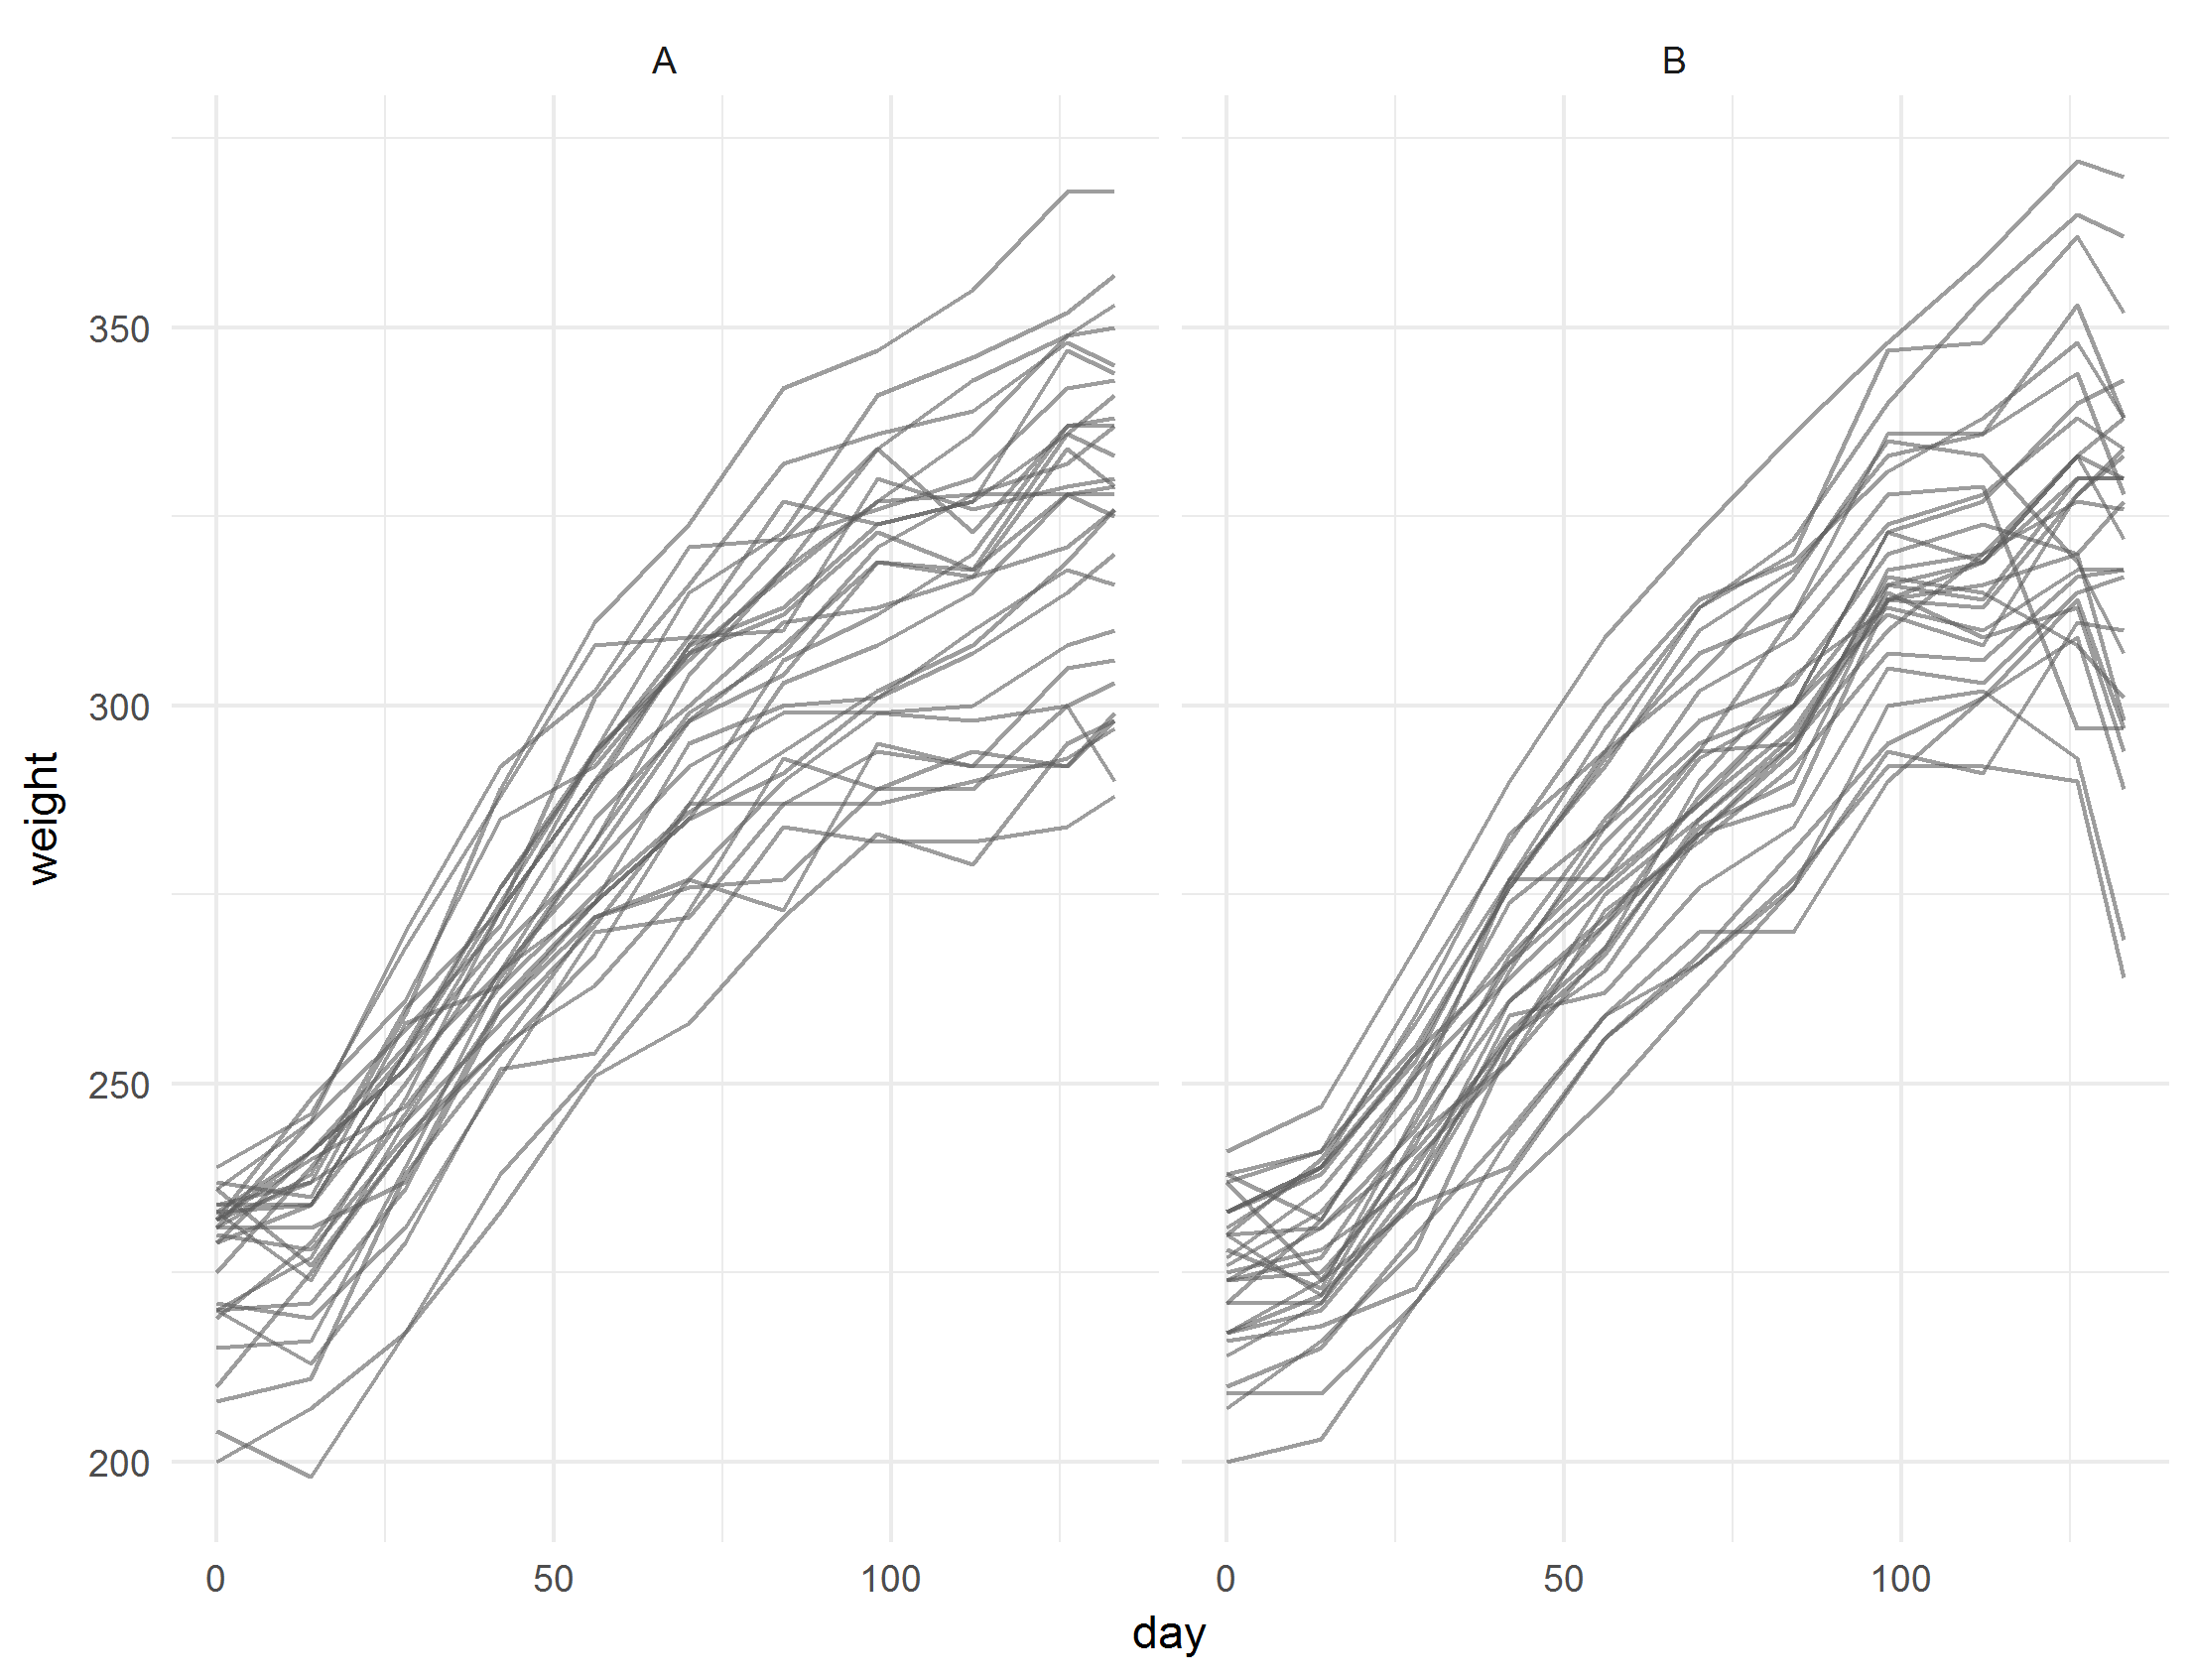
\includegraphics[width = \textwidth]{img/cattle/cattle-weights-vs-time-by-trt}
\end{center}
\end{figure} 

We see an upward trend in weights over time, with variance in weights increasing over time for both groups. Treatment group B demonstrates a sharp decrease in the final weight measurement. The analysis of the same dataset provided by \cite{zimmerman1997structured} rejected equality of the two covariance matrices corresponding to treatment group using the classical likelihood ratio test, making it reasonable to study each treatment group's covariance matrix separately. Following \cite{pan2017jmcm}, \cite{zhang2015joint}, \cite{pourahmadi1999joint}, and \cite{pan2006regression}, we analyze the data from the $N = 30$ cattle assigned to treatment group A, which we assume share a common $11 \times 11$ covariance matrix $\Sigma$. The profile plot in Figure~\ref{fig:cattleA-weights-vs-time} of the weights for units in treatment group A shows a clear upward trend in weights;  variances appear to increase over time, suggesting that the covariance structure is nonstationary.

\bigskip

Before modeling the covariance structure, it is necessary to construct an adequate estimate of the mean weight trajectories. After centering the data using the fitted mean, the residuals serve as the data reserved for estimating the functions defining the Cholesky factor and innovation variances.  To account for any between-subject variability, we adopt an approach akin to the dynamical conditionally linear mixed model proposed by Pourahmadi and Daniels; see \cite{pourahmadi2002dynamic} for a detailed discussion. We model

\begin{equation} \label{eq:cattleA-dynamic-cond-mixed-model-1}
r\left(t_{ij}\right) = \sum_{k < j} \phi\left( t_{ij}, t_{ik} \right) r\left(t_{ij}\right) + \epsilon\left(t_{ij}\right)
\end{equation}
\noindent
where
\begin{equation} \label{eq:cattleA-dynamic-cond-mixed-model-2}
r\left(t_{ij}\right) = y\left(t_{ij}\right) - \left(f\left(t_{ij} \right) + \alpha_{i}\right).
\end{equation}
\noindent
The subject-specific random effects $\left\{ \alpha_i \right\}$ are assumed to be mutually independent and independent of $ \epsilon\left(t_{ij}\right)$ for all $i,\;j$, with

\[
\alpha_i \sim N\left( 0, \sigma_\alpha^2 \right).
\]
\noindent
We assume that the subject trajectories share a common mean function $f \in $

\[
\mathcal{C}^2 = \left\{f: \; f,\;f' \mbox{ absolutely continuous, } \int\left(f''\left(x\right)\right)^2 \;dx < \infty  \right\}.
\]
\noindent
Figure~\ref{fig:cattleA-weights-vs-time} displays the he observed weight trajectories over time. Figure~\ref{fig:cattleA-smoothed-weights-vs-time} shows the corresponding fitted mean curves.

\begin{figure}[H] \label{fig:cattleA-weights-vs-time}
\begin{center}
    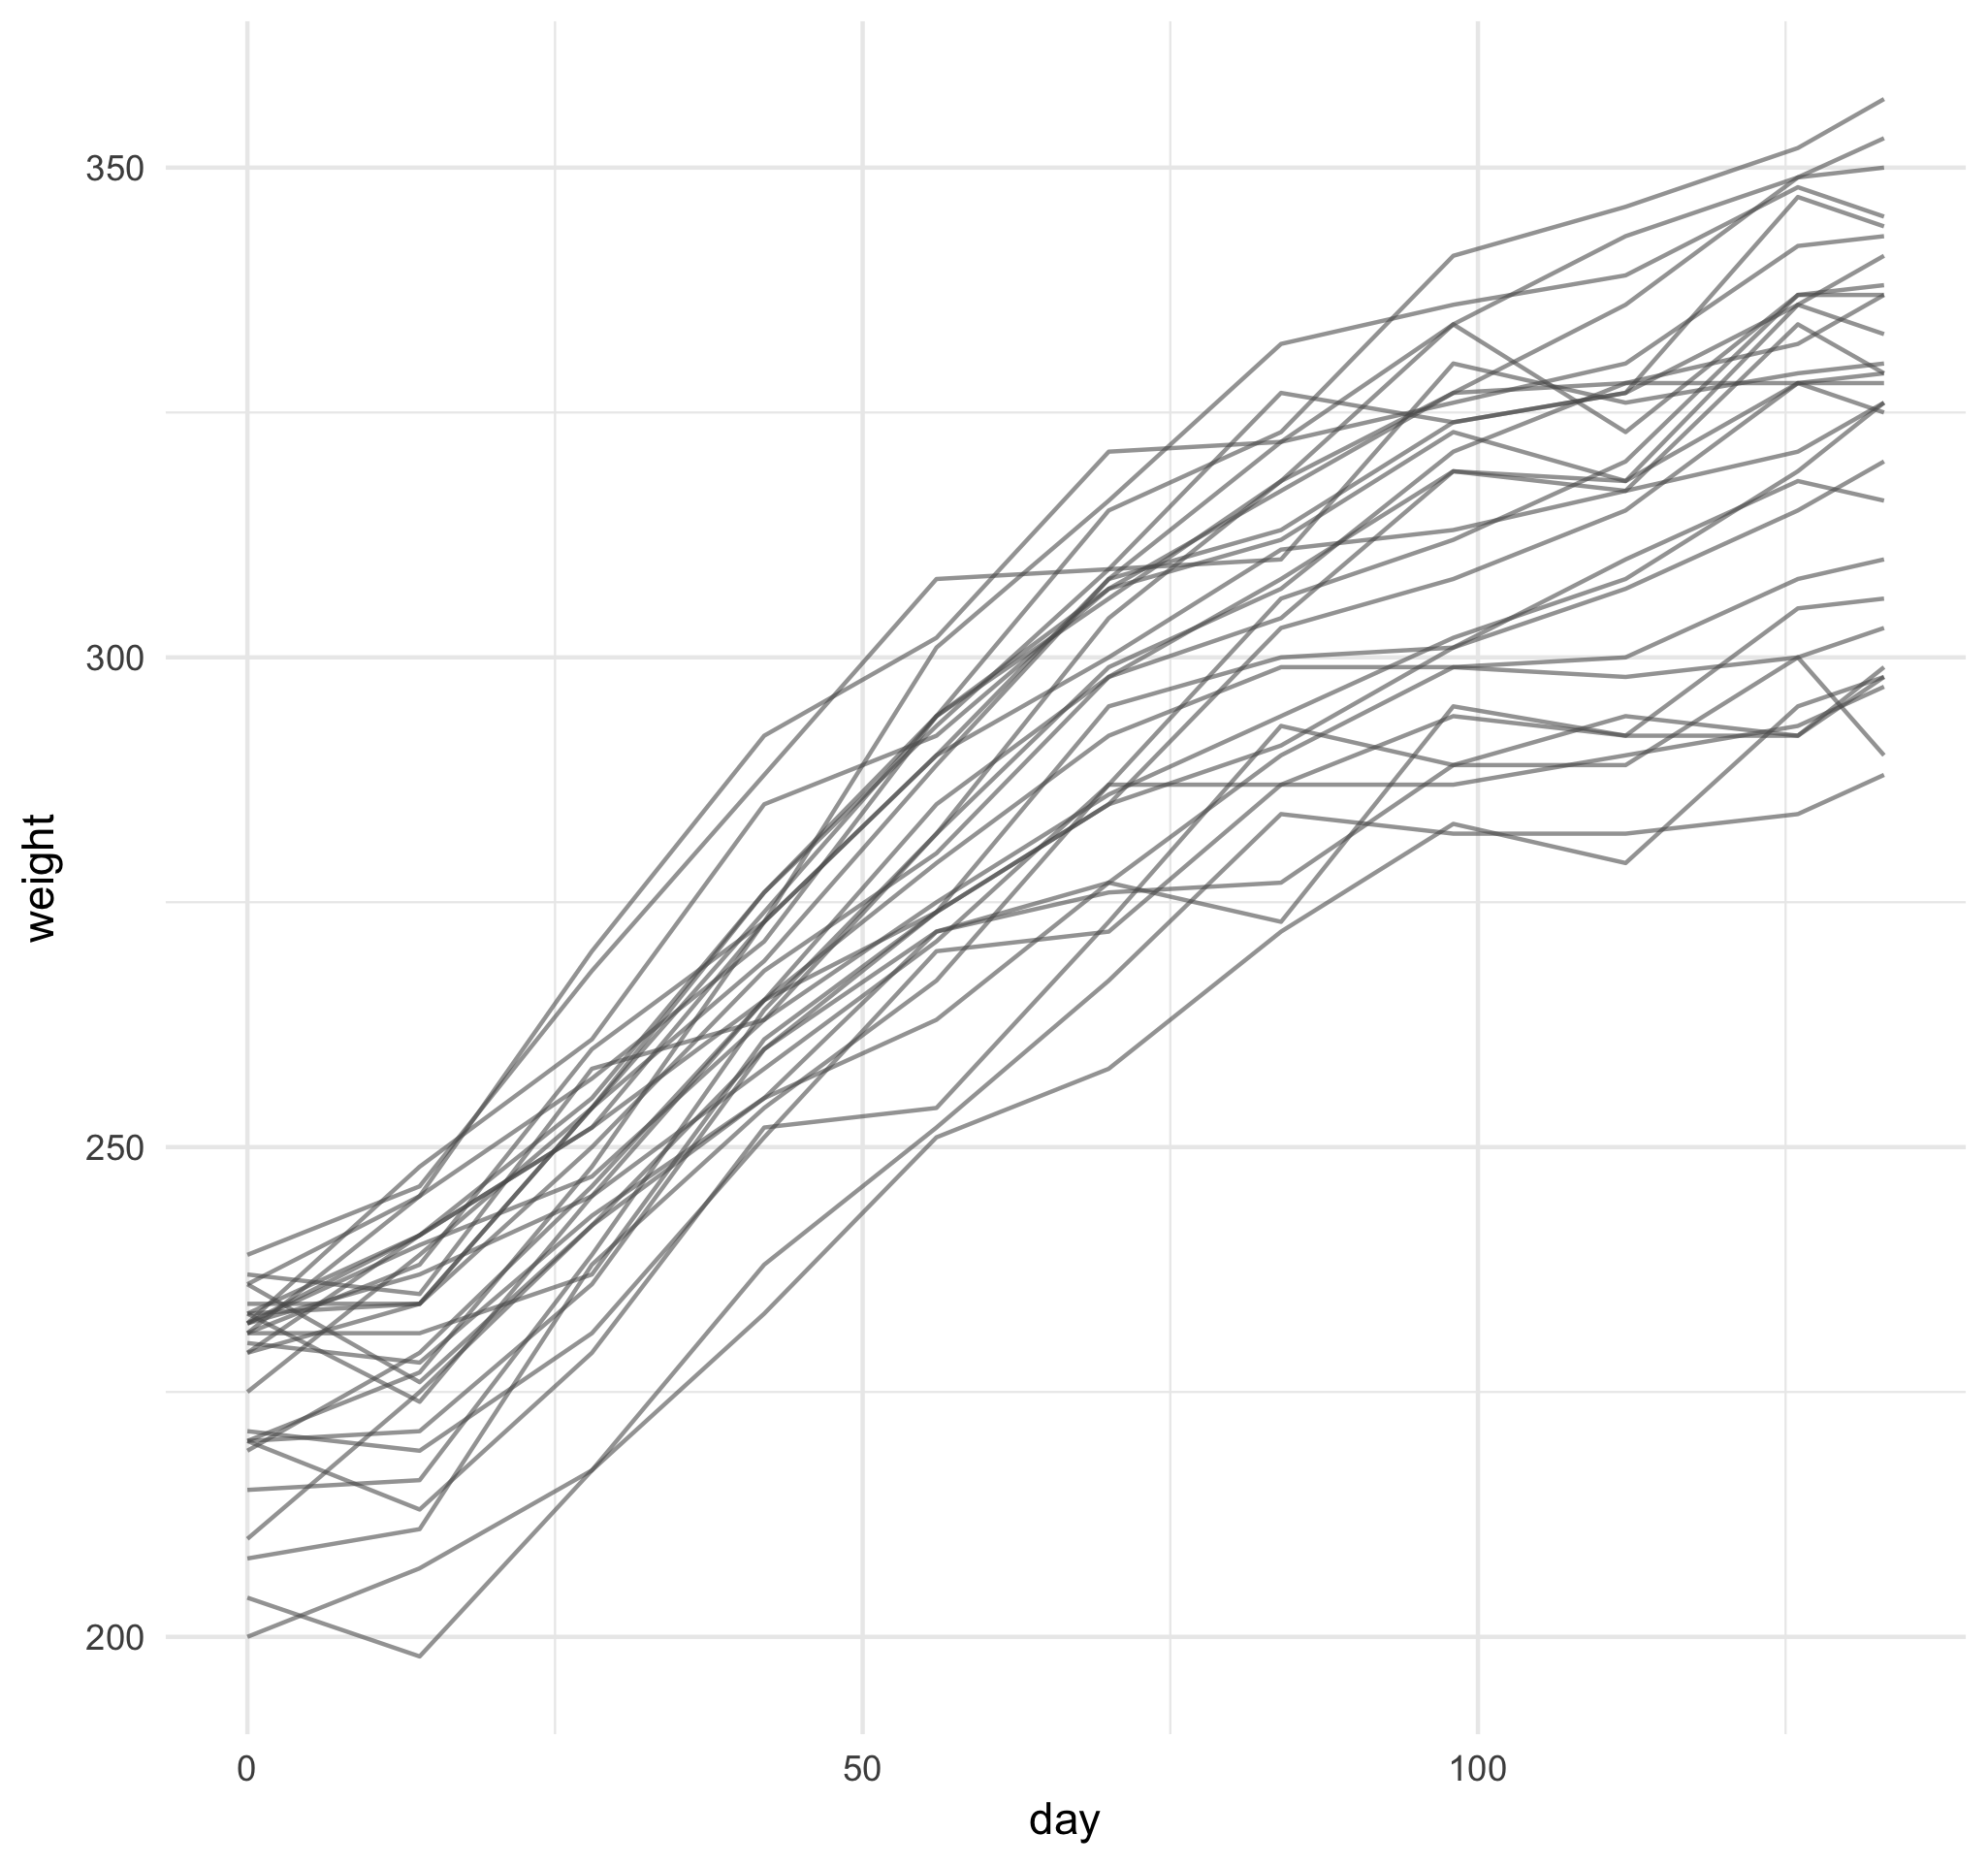
\includegraphics[width=\textwidth]{img/cattle/cattleA-weights-vs-time}
\end{center}
 \caption{Weight trajectories over the observation period for experimental units in treatment group A.}
 \end{figure}

\begin{figure}[H] \label{fig:cattleA-smoothed-weights-vs-time}
\caption{Fitted mean weight curve for cattle in treatment group A. }
\begin{center}
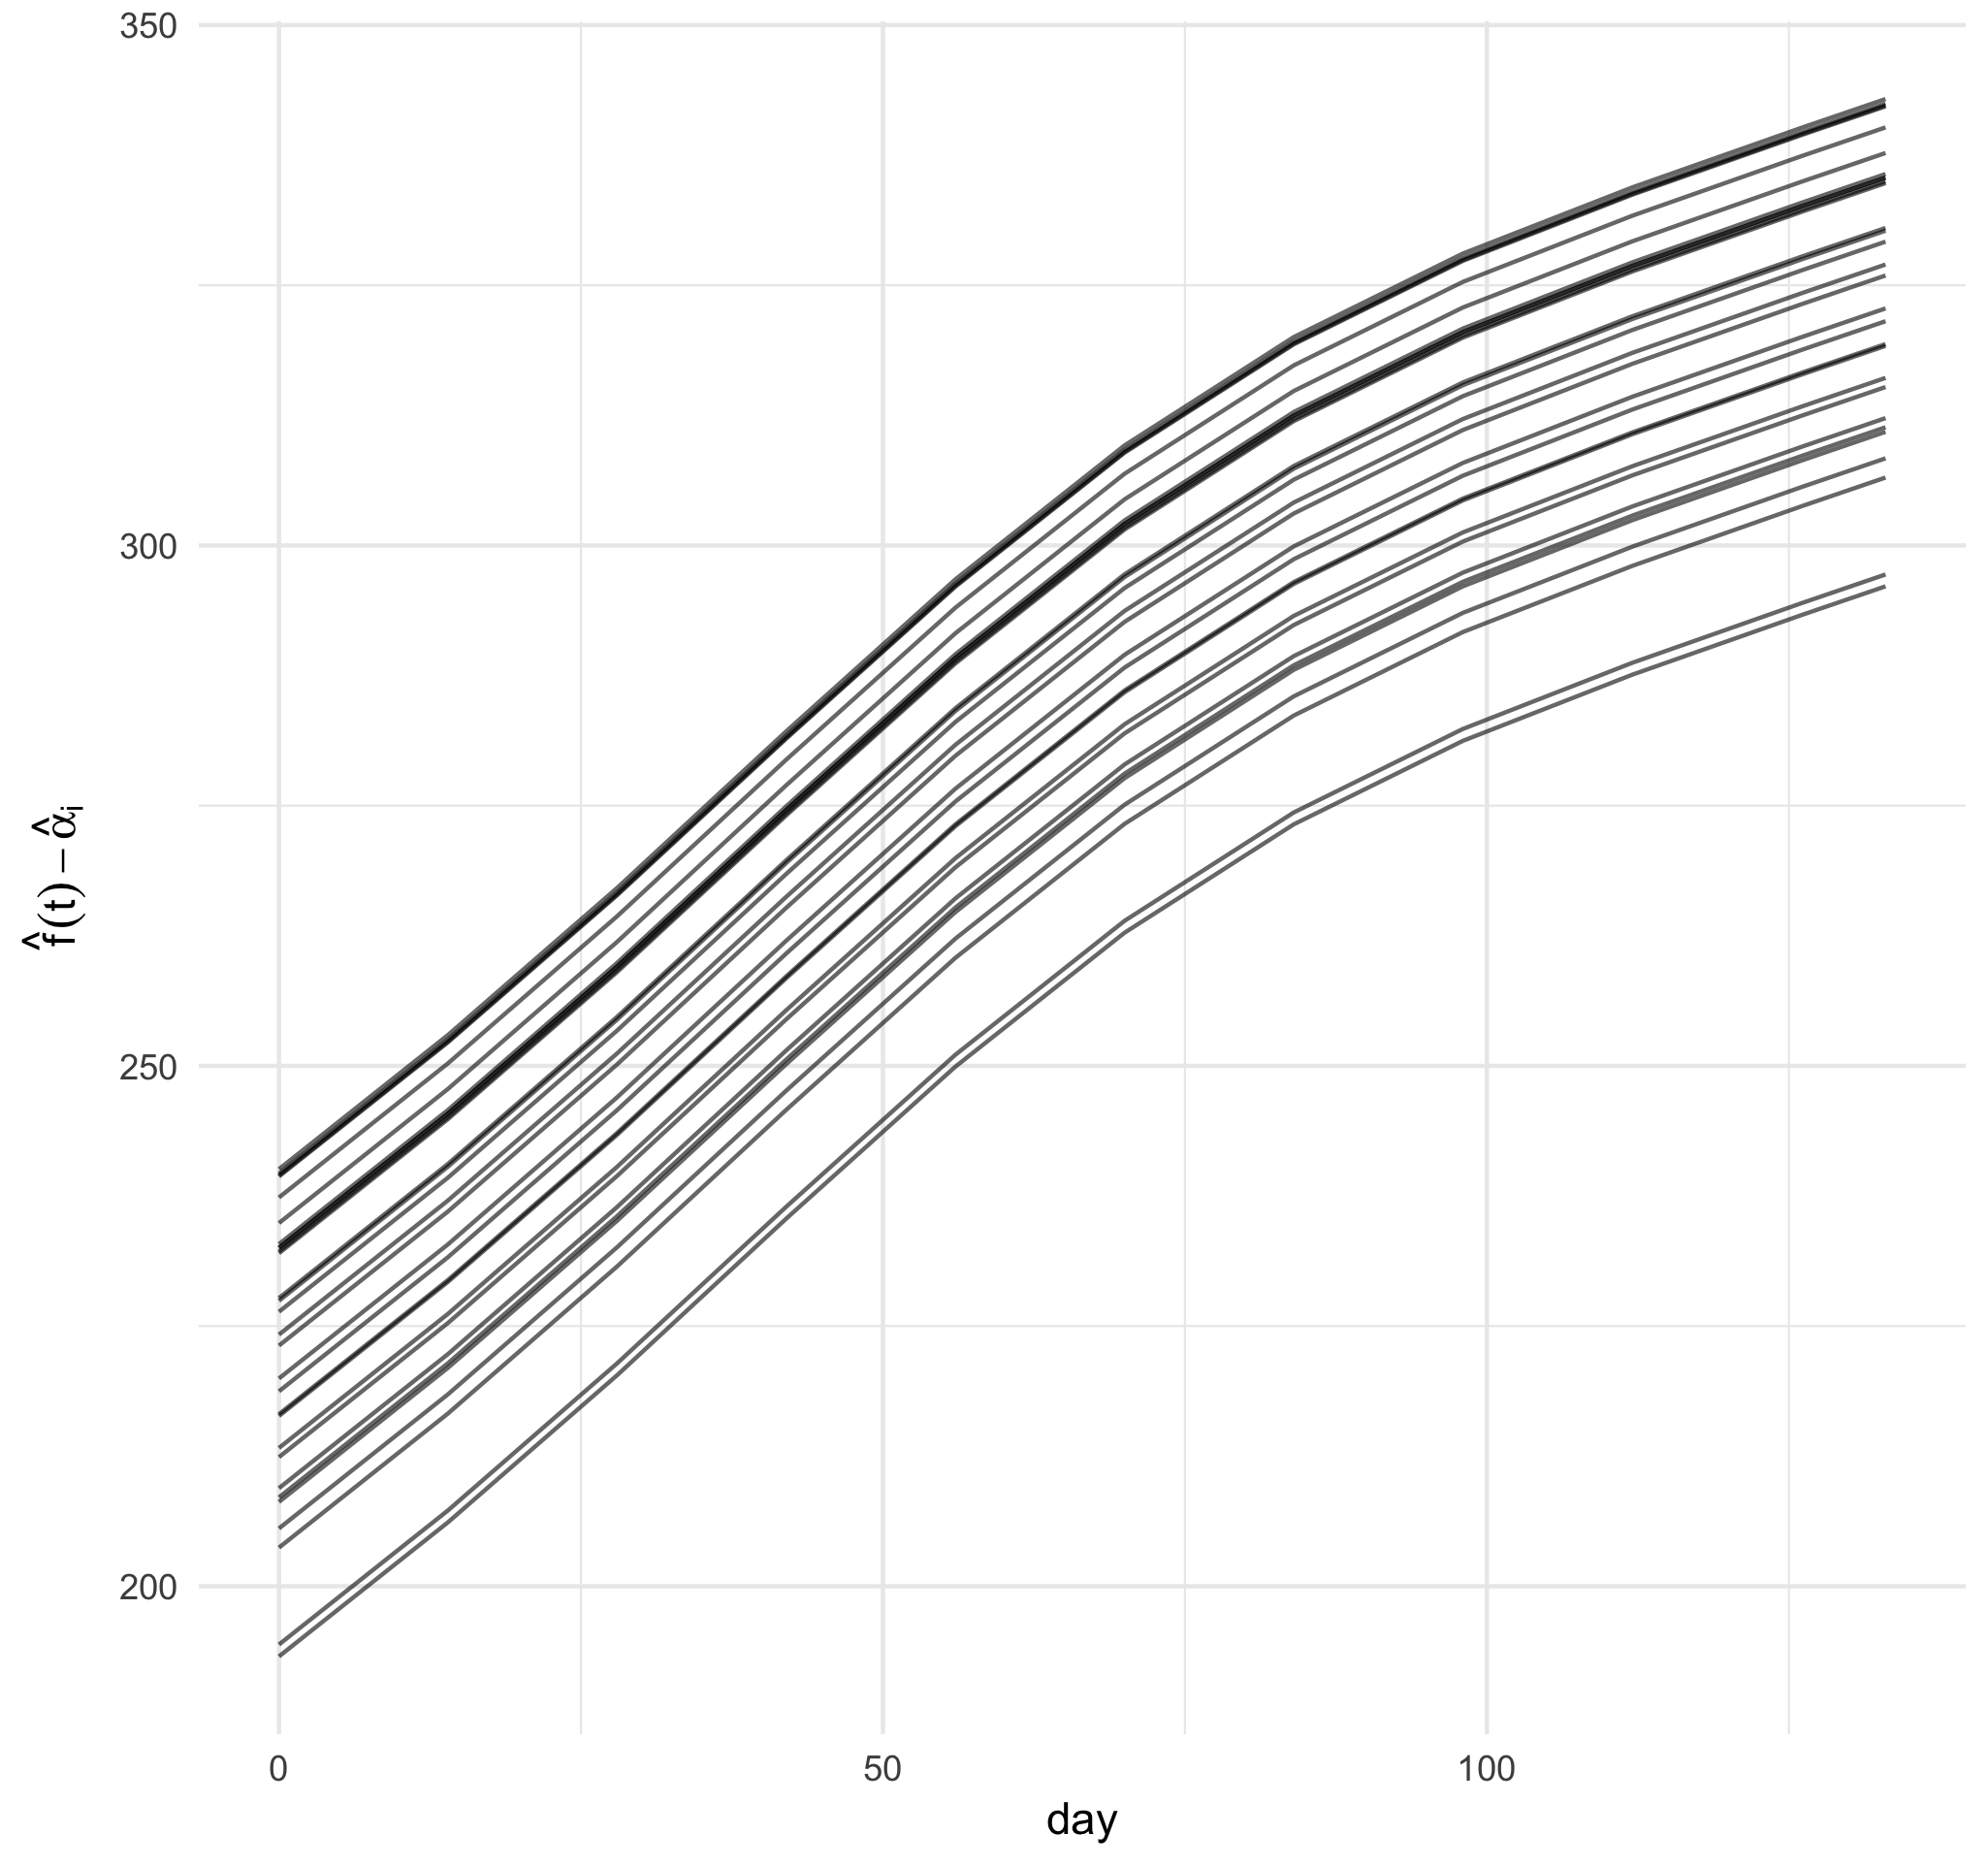
\includegraphics[width = \textwidth]{img/cattle/cattleA-weights-vs-time-mean-fit}
\end{center}
\end{figure} 

The nonstationarity suggested in Figure~\ref{fig:cattle-weights-by-trt} is also supported by the sample correlations given in Table~\ref{table:cattleA-sample-correlations}; correlations within the subdiagonals are not constant and increase over time, a secondary indication that a stationary covariance is not appropriate for the data.  Table~\ref{table:sample-regressogram-garps} gives the sample generalised autoregressive parameters and the innovation variances, which are plotted in Figure~\ref{fig:cattleA-regressogram} and Figure~\ref{fig:cattleA-innovation-variogram} respectively. 

\begin{table}[H] \label{table:cattleA-sample-correlations}
\begin{center}
\begin{tabular}{r|rrrrrrrrrrr}
& \multicolumn{11}{c}{day}\\
 & 0 & 14 & 28 & 42 & 56 & 70 & 84 & 98& 112& 126 &133\\ 
  \hline
0 & 1.00 & 0.82 & 0.76 & 0.65 & 0.63 & 0.58 & 0.51 & 0.52 & 0.51 & 0.46 & 0.46 \\ 
  14 & 0.82 & 1.00 & 0.91 & 0.86 & 0.83 & 0.75 & 0.64 & 0.68 & 0.61 & 0.59 & 0.56 \\ 
  28 & 0.76 & 0.91 & 1.00 & 0.93 & 0.89 & 0.85 & 0.75 & 0.77 & 0.71 & 0.69 & 0.67 \\ 
  42 & 0.65 & 0.86 & 0.93 & 1.00 & 0.93 & 0.90 & 0.80 & 0.82 & 0.74 & 0.70 & 0.67 \\ 
  56 & 0.63 & 0.83 & 0.89 & 0.93 & 1.00 & 0.94 & 0.85 & 0.88 & 0.81 & 0.77 & 0.74 \\ 
  70 & 0.58 & 0.75 & 0.85 & 0.90 & 0.94 & 1.00 & 0.92 & 0.93 & 0.89 & 0.85 & 0.81 \\ 
  84 & 0.51 & 0.64 & 0.75 & 0.80 & 0.85 & 0.92 & 1.00 & 0.92 & 0.92 & 0.86 & 0.84 \\ 
  98 & 0.52 & 0.68 & 0.77 & 0.82 & 0.88 & 0.93 & 0.92 & 1.00 & 0.96 & 0.94 & 0.91 \\ 
  112 & 0.51 & 0.61 & 0.71 & 0.74 & 0.81 & 0.89 & 0.92 & 0.96 & 1.00 & 0.96 & 0.95 \\ 
  120 & 0.46 & 0.59 & 0.69 & 0.70 & 0.77 & 0.85 & 0.86 & 0.94 & 0.96 & 1.00 & 0.98 \\ 
  133 & 0.46 & 0.56 & 0.67 & 0.67 & 0.74 & 0.81 & 0.84 & 0.91 & 0.95 & 0.98 & 1.00 \\ 
   \hline
\end{tabular}
\caption{Cattle data: treatment group A sample correlations.}
\end{center}
\end{table}


\begin{table}[ht] \label{table:sample-regressogram-garps}
\begin{center}
\begin{tabular}{lc|ccccccccccc|cr}
& \multicolumn{11}{c}{s}\\
&&&&&&&&&&&&\\
& & 1 & 2 & 3 & 4 & 5 & 6 & 7 & 8 & 9 & 10 & 10.5 & \\ 
  \hline
&1 & 1 & &&&&&&&&& & 4.673& \\ 
&  2 & 1.00 & $\ddots$&&&&&&&&&& 3.939 &\\ 
&  3 & 0.04 & 0.90 &  &&&&&&&&& 3.370&\\ 
&  4 & -0.25 & 0.25 & 0.88 &  &&&&&&&&3.000& \\ 
&  5 & -0.02 & 0.07 & 0.12 & 0.90 & &&&&&&& 3.299&\\ 
t &  6 & 0.04 & -0.28 & 0.11 & 0.37 & 0.82  &&&&&&& 3.363 & $\log\left(\sigma^2_t\right)$\\ 
 & 7 & 0.12 & -0.23 & 0.04 & -0.16 & 0.08 & 1.03  &&&&&& 3.610\\ 
 & 8 & -0.06 & 0.05 & 0.02 & -0.27 & 0.23 & 0.61 & 0.42 &&&&& 3.403&\\ 
 & 9 & 0.18 & -0.10 & 0.05 & -0.26 & -0.10 & 0.03 & 0.30 & 0.93&&&& 2.780&  \\ 
 & 10 & -0.26 & 0.15 & 0.45 & -0.33 & -0.19 & 0.01 & -0.18 & 0.37 & 0.94 & $\ddots$&&3.280& \\ 
 & 10.5 & 0.13 & -0.26 & 0.08 & 0.28 & 0.04 & -0.36 & -0.05 & -0.07 & 0.37 & 0.85 & 1  &2.262&\\ 
\end{tabular}
\caption{Cattle data: treatment group A sample generalized autoregressive parameters (below the main diagonal) and log sample innovation variances (rightmost column.)}
\end{center}
\end{table}


\begin{figure}[H]
 \begin{subfigure}{.48\textwidth}
  \centering
    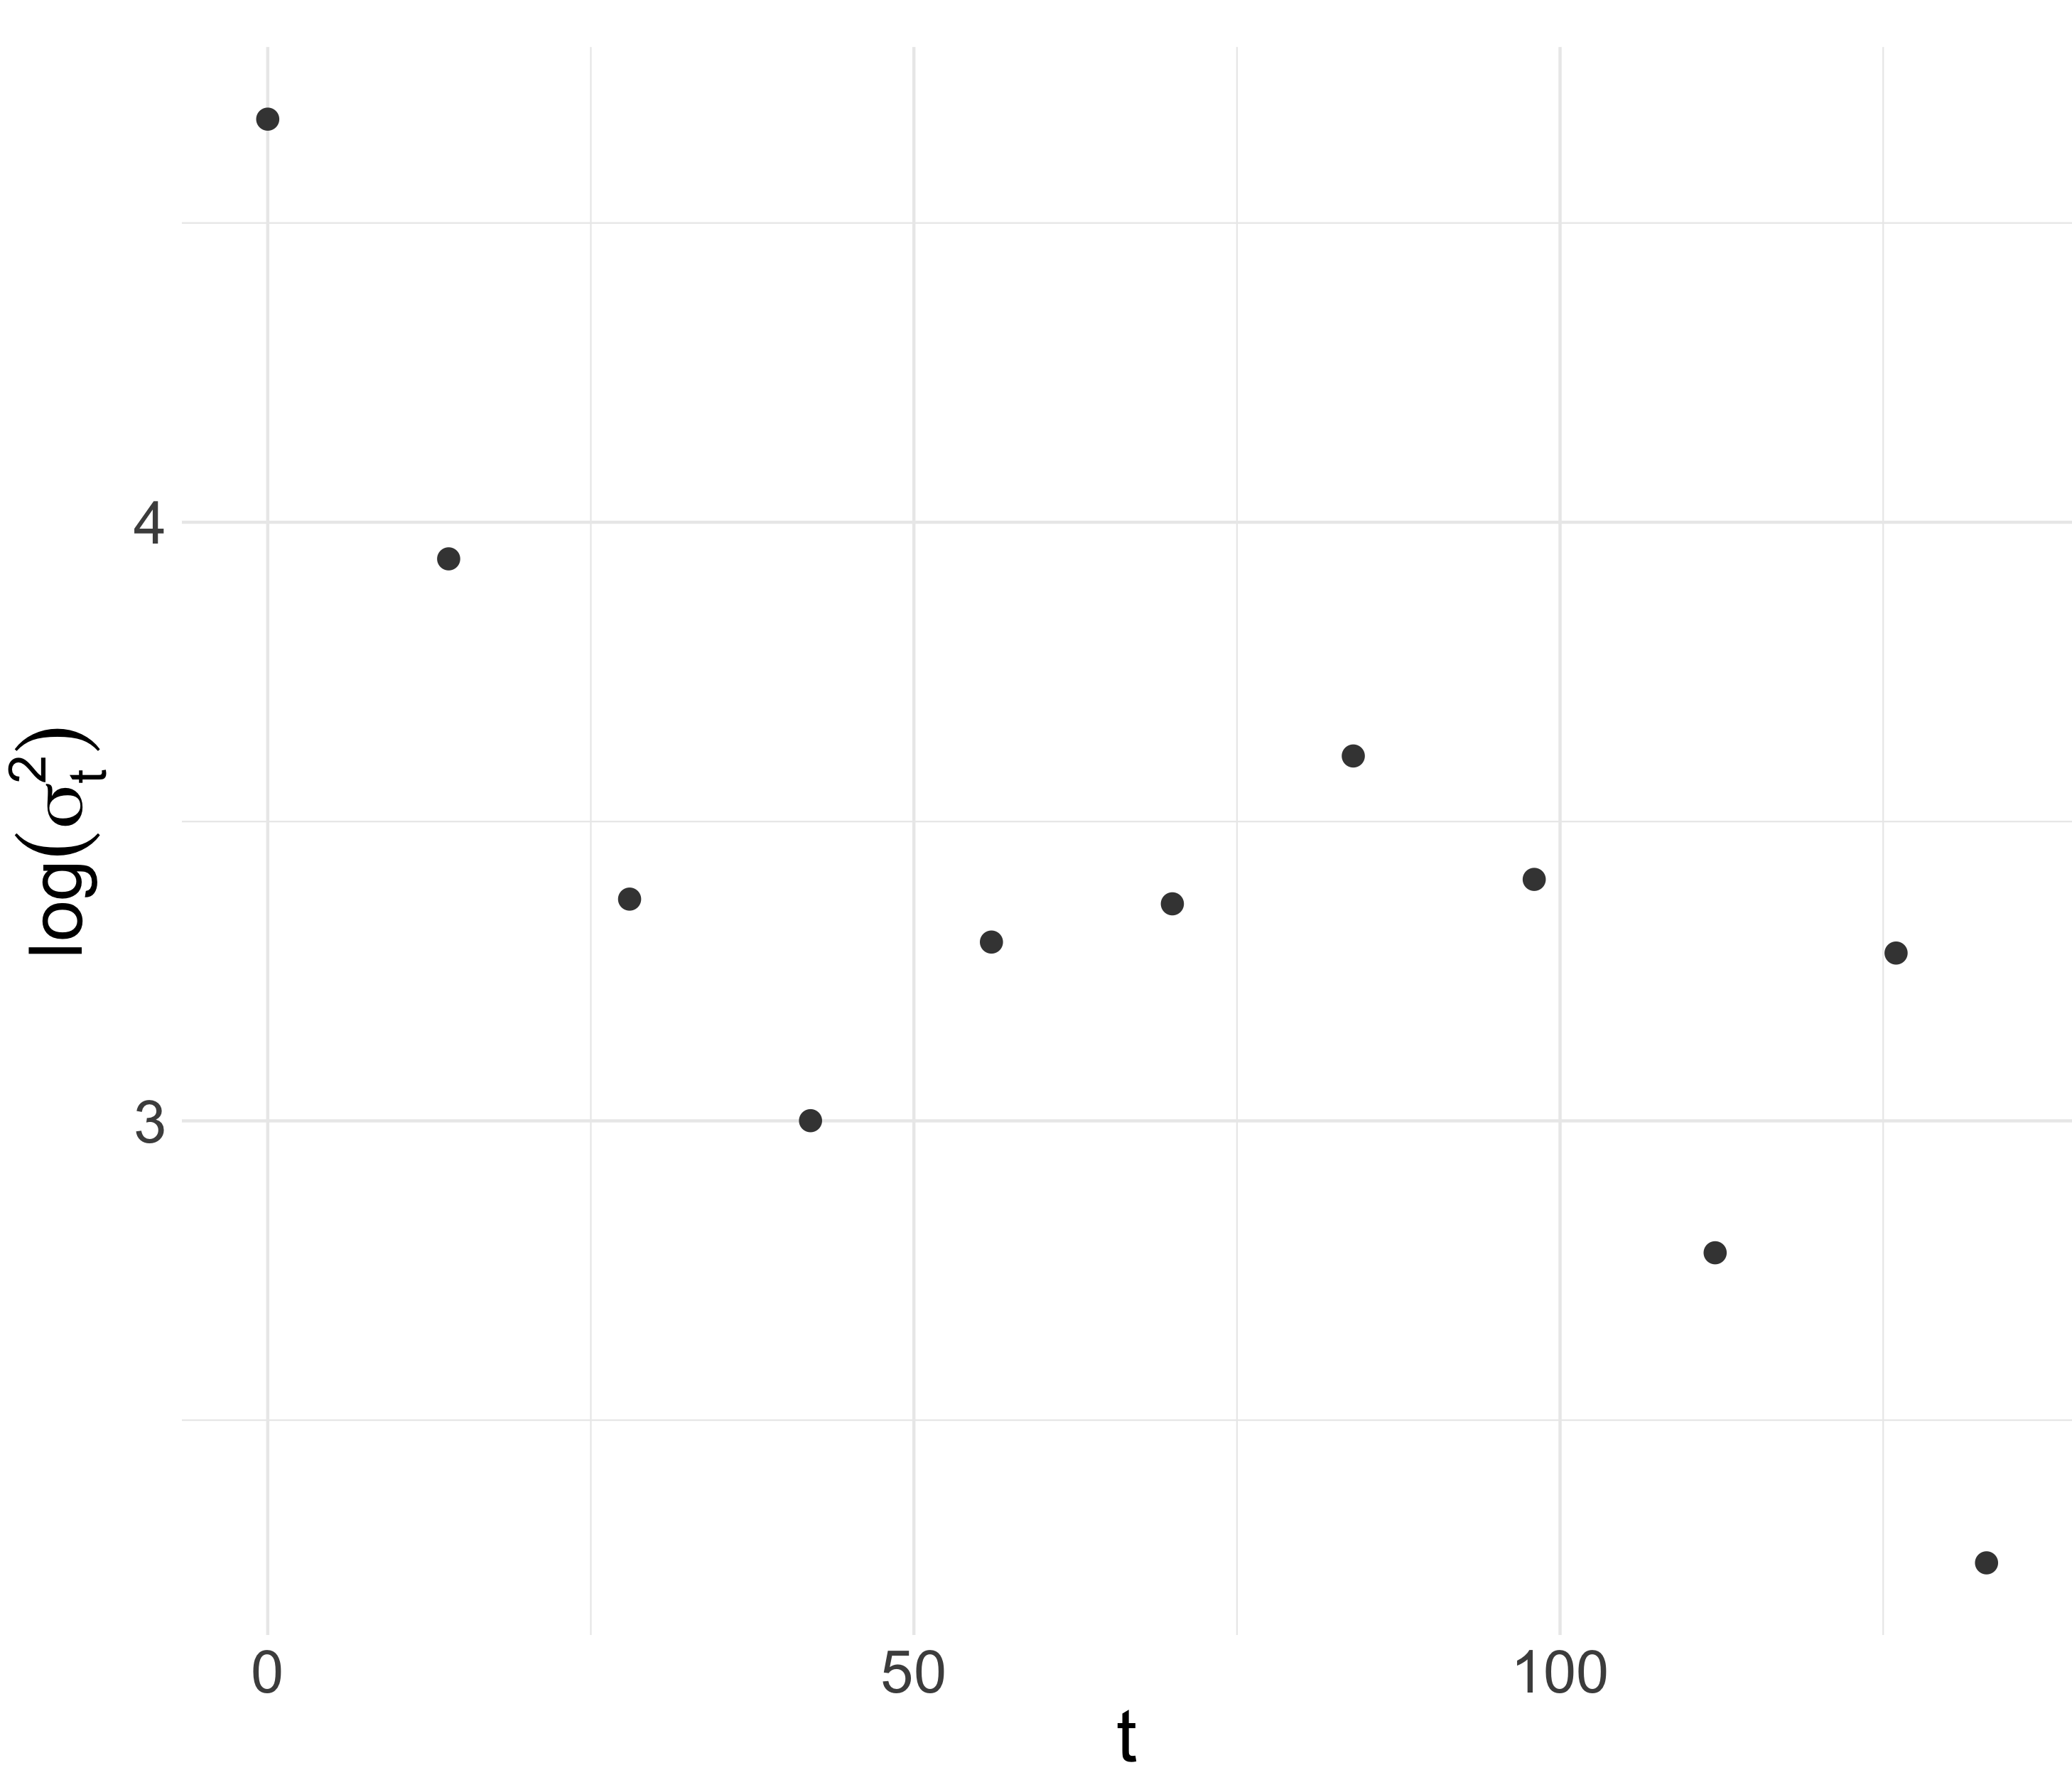
\includegraphics[width=\textwidth]{img/cattle/cattleA-innovation-variogram}
 \caption{Sample estimates of innovation variances $\sigma_t^2$ obtained by applying the modified Cholesky decomposition to the sample covariance matrix.} \label{fig:cattleA-innovation-variogram}
 \end{subfigure}
 \begin{subfigure}{.48\textwidth}
  \centering
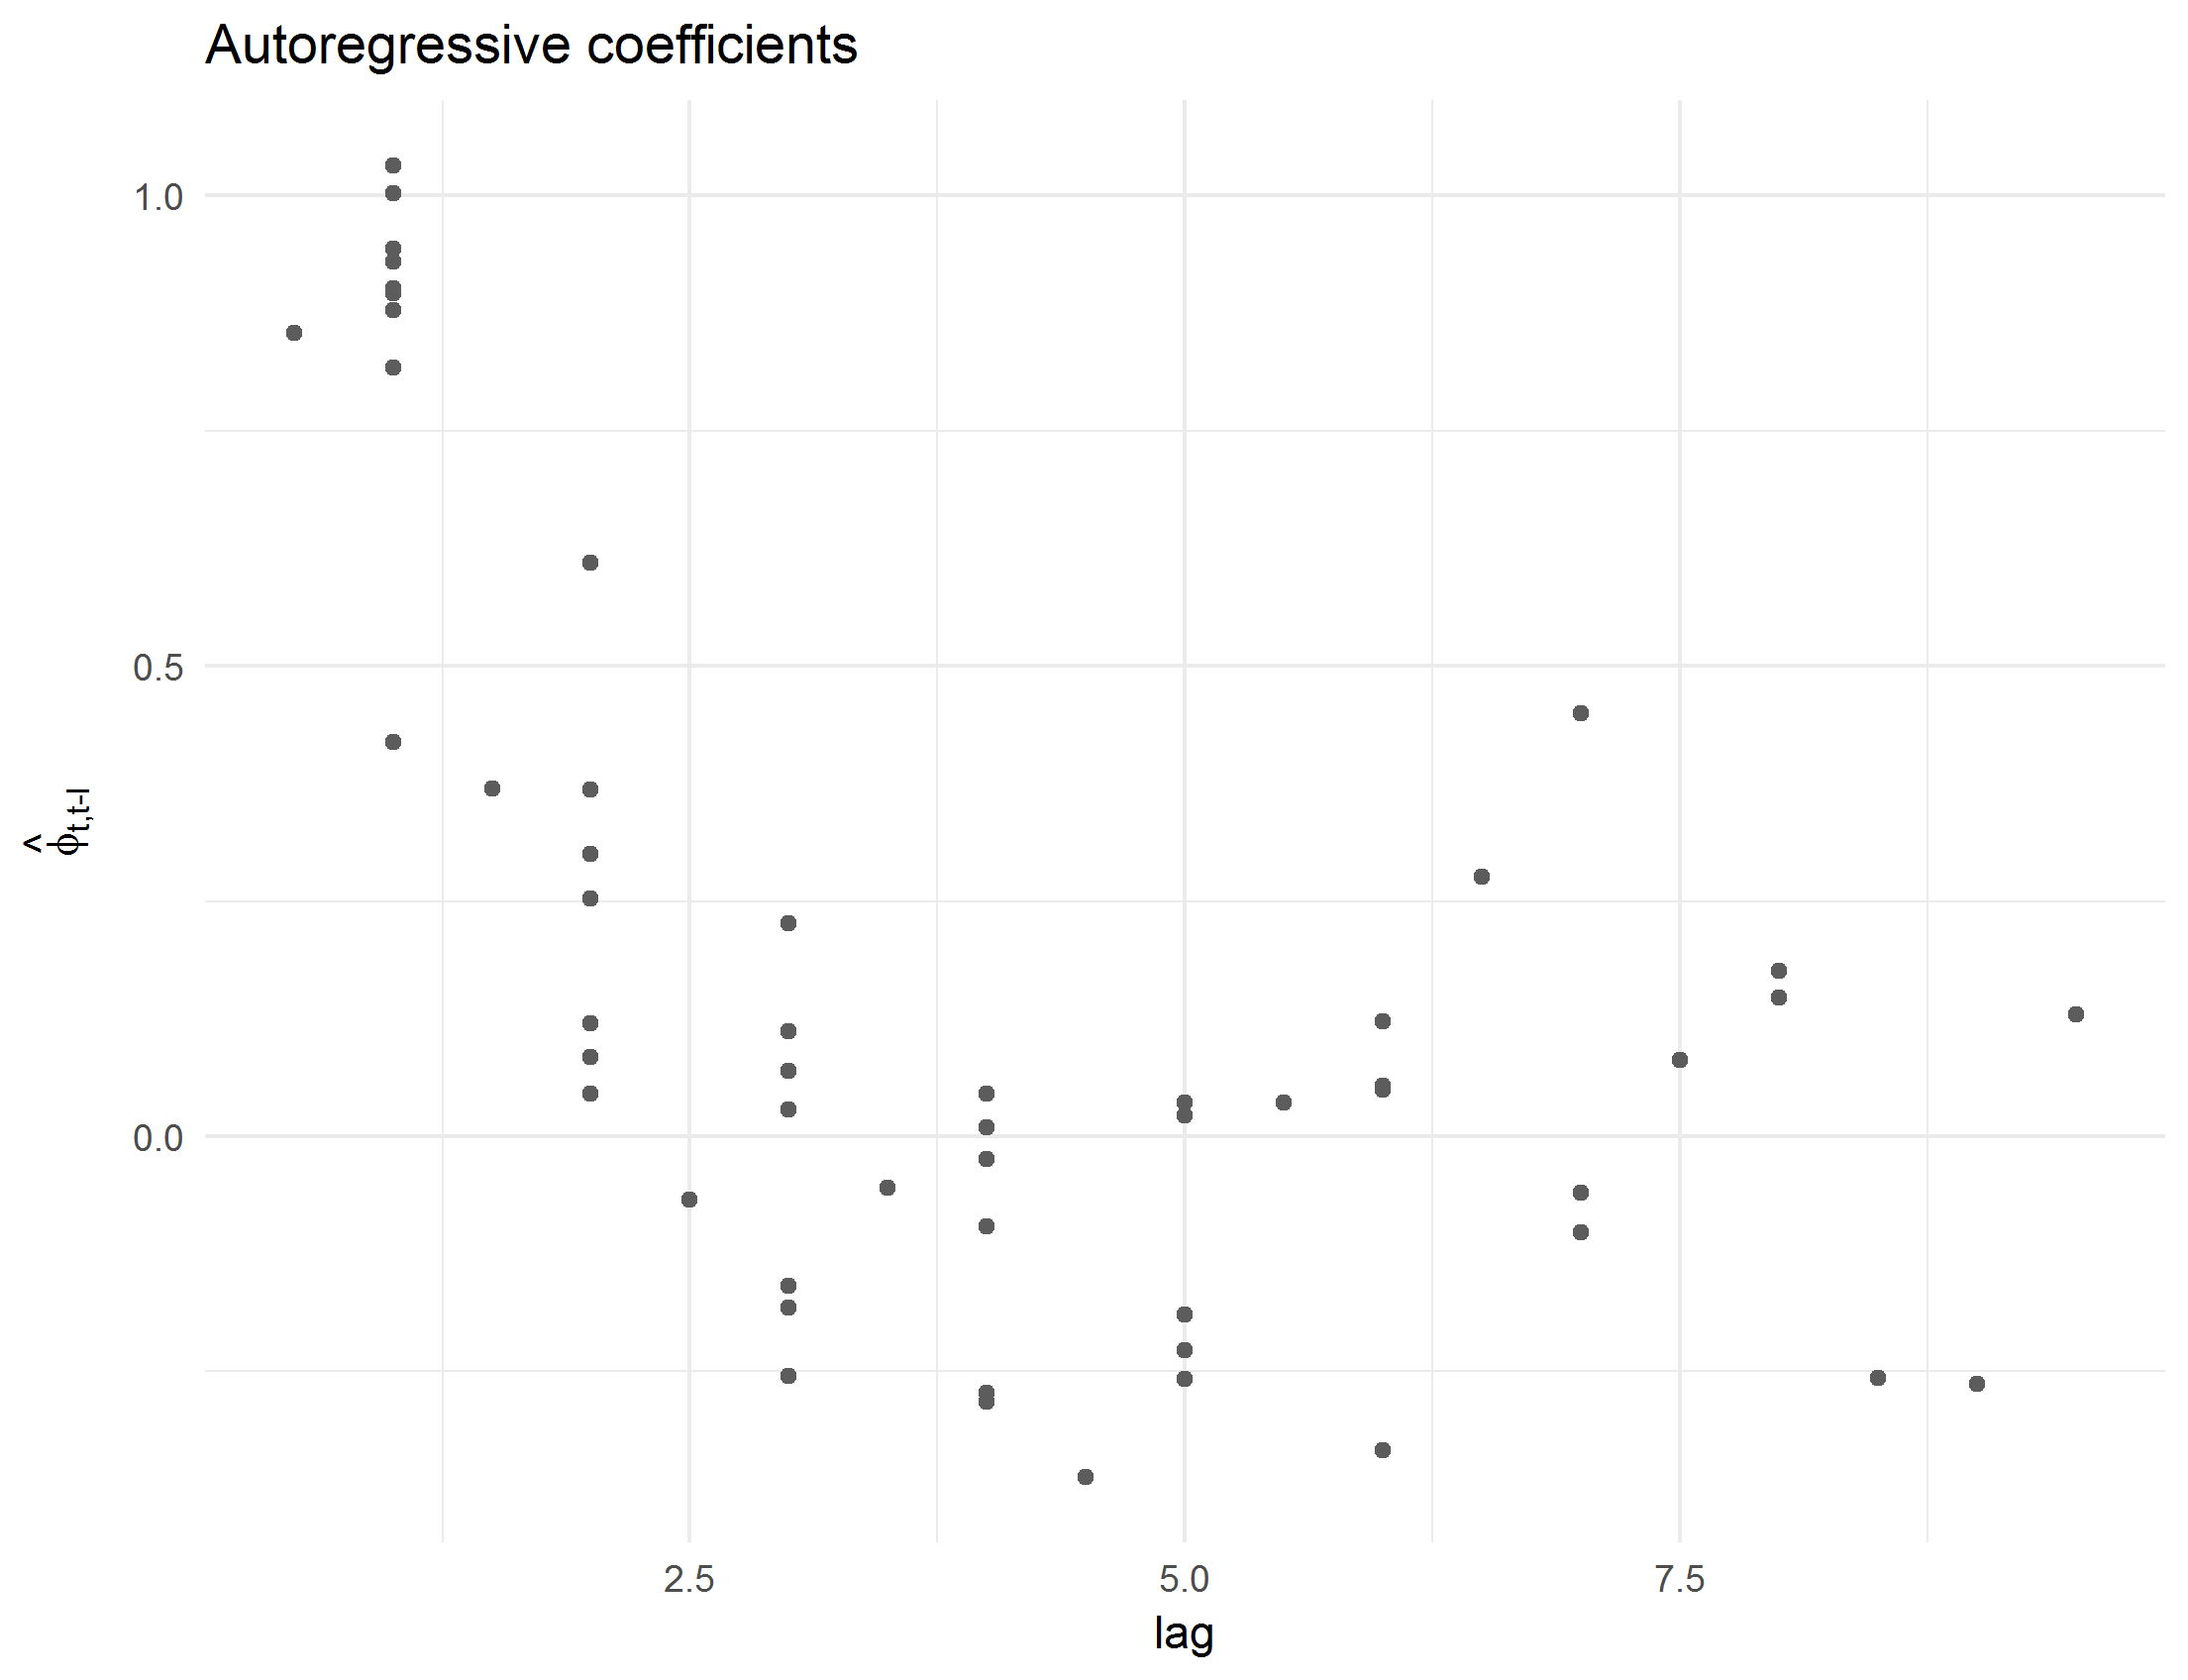
\includegraphics[width = \textwidth]{img/cattle/cattleA-regressogram}
 \caption{Sample estimates of the generalized autoregressive parameters $\phi_{ij}$ obtained by applying the modified Cholesky decomposition to the sample covariance}
\label{fig:cattleA-regressogram}
 \end{subfigure}
% \caption{\textit{Estimated coefficient function} $\hat{\beta}\left(t\right)$ \textit{and mean curve} $\hat{\mu}\left(t\right) = t \sin(2 \pi t)$ \textit{using a 80 B-splines basis functions of order 5 and a difference penalty of order} $k=3$.}
\end{figure}

%
%\begin{figure}[H] \label{fig:cattleA-innovation-variogram}
%\begin{center}
%    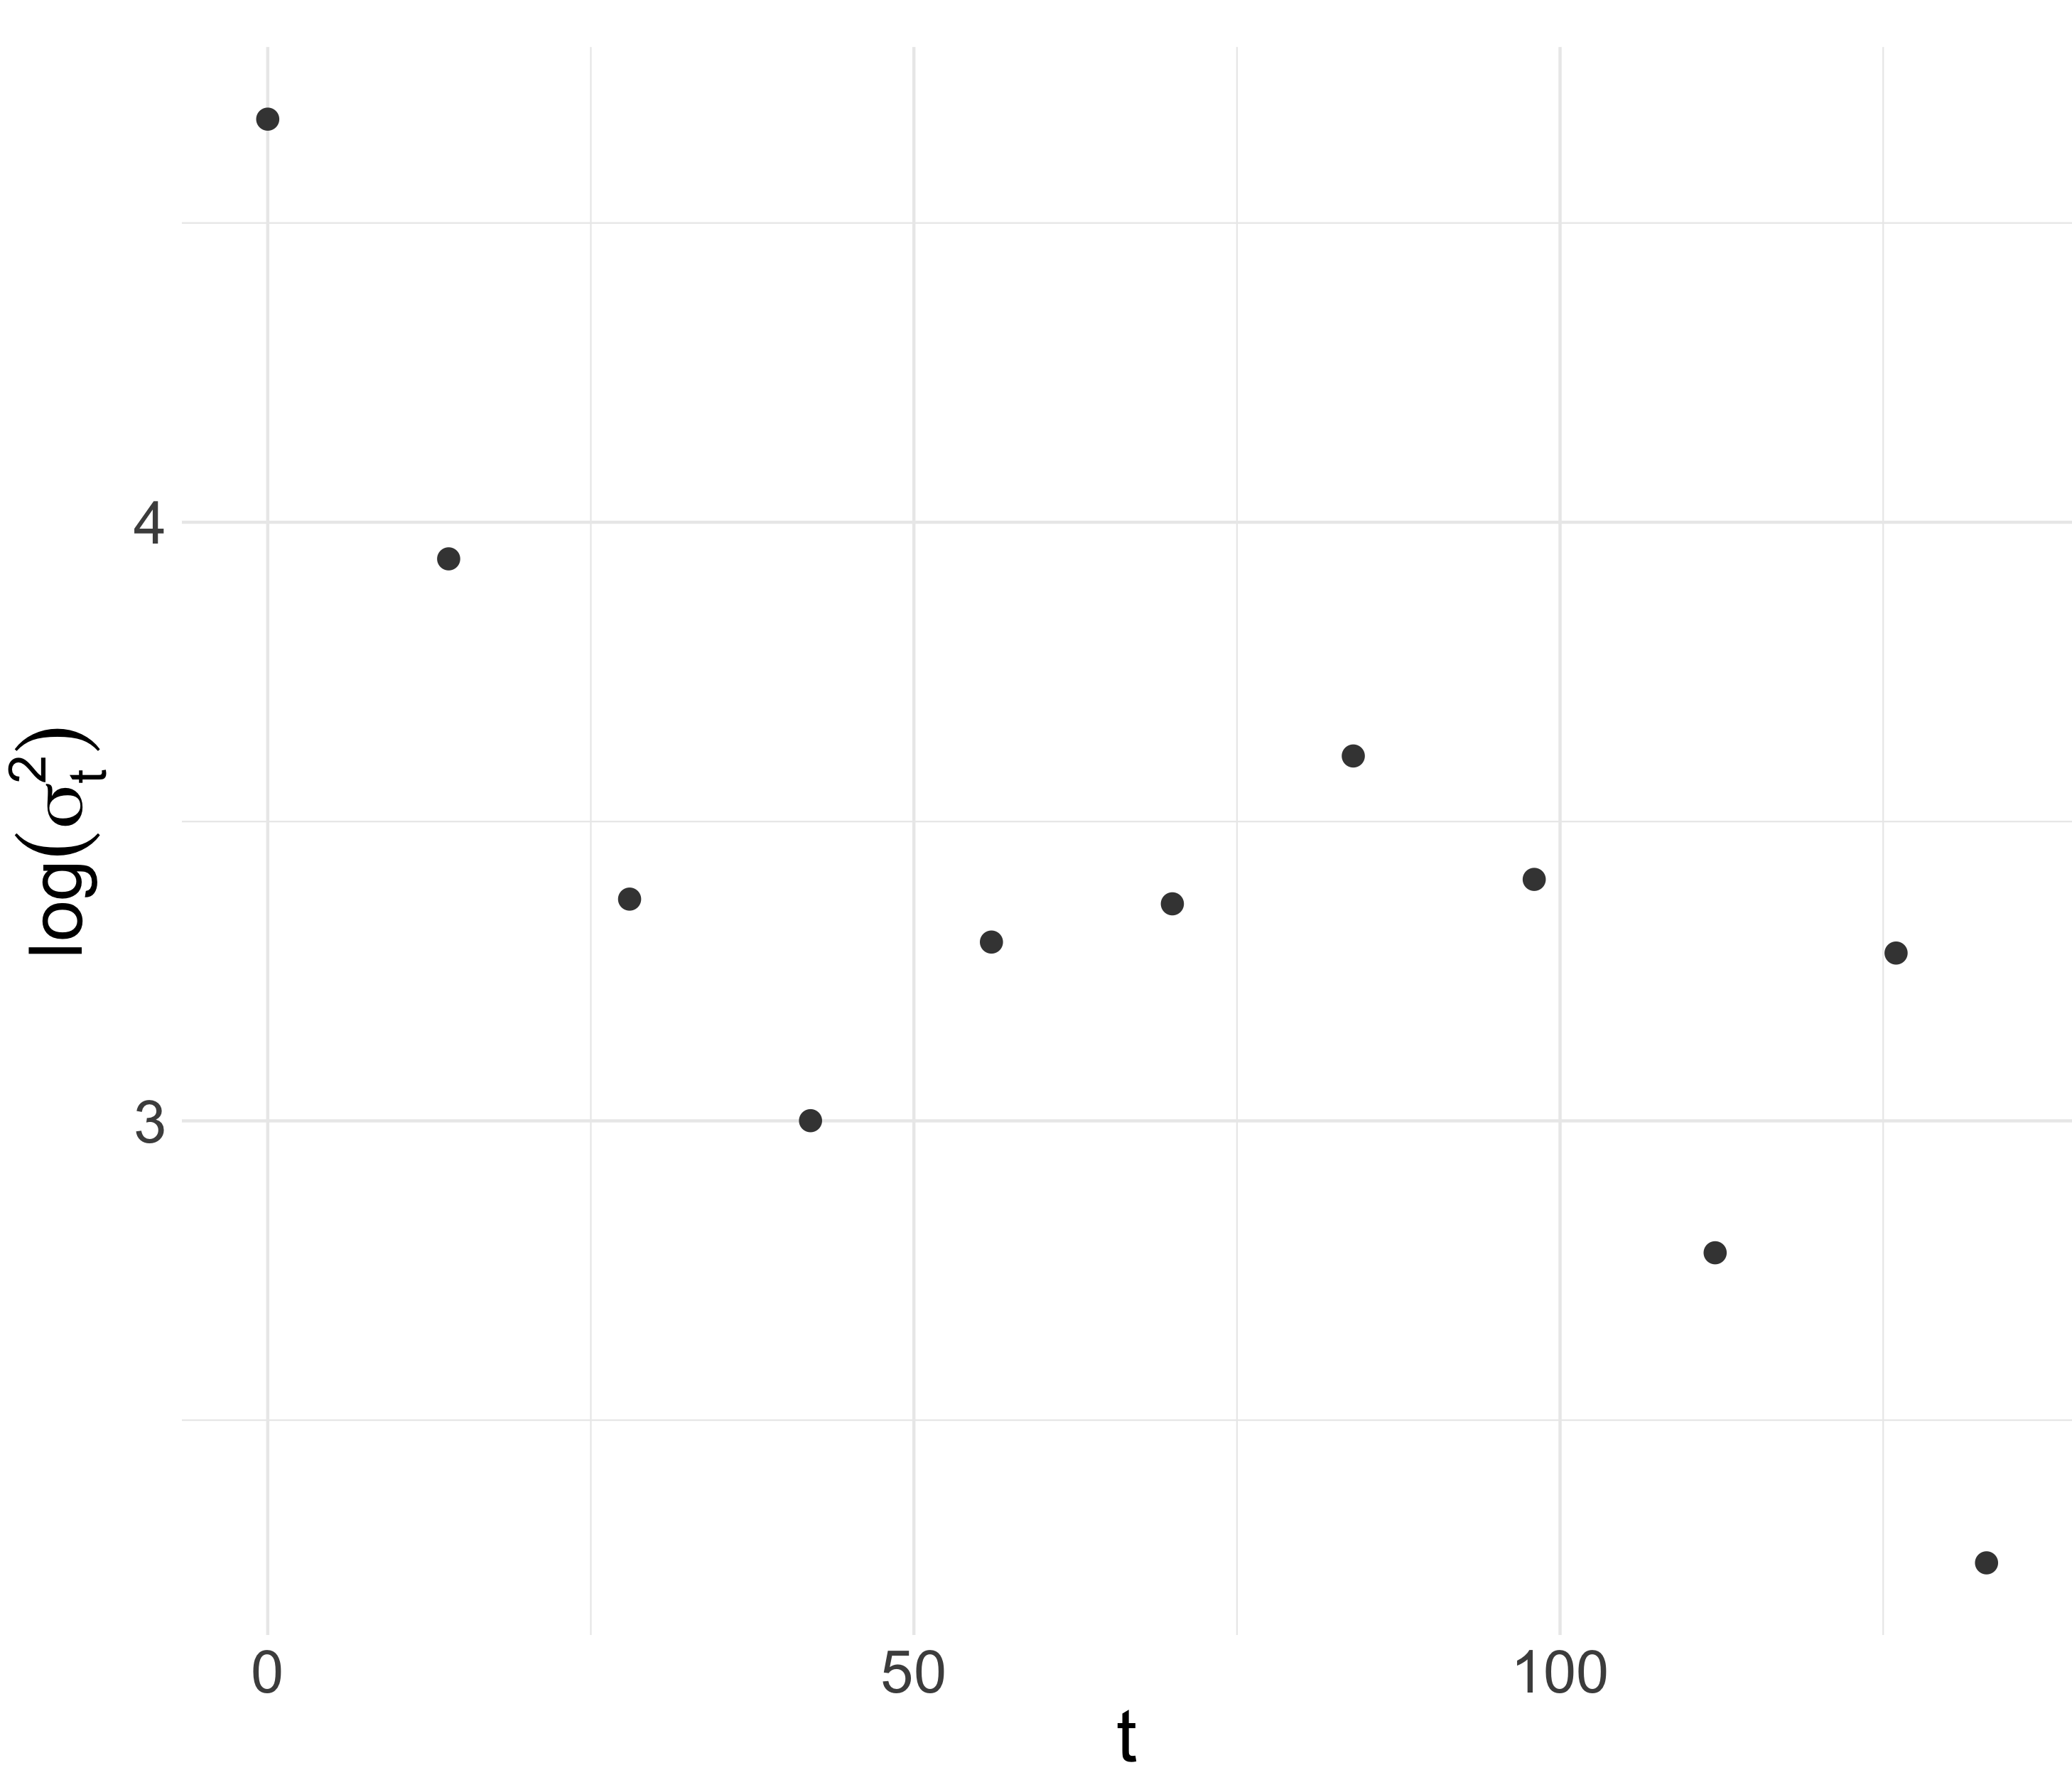
\includegraphics[width=\textwidth]{img/cattle/cattleA-innovation-variogram}
%\end{center}
% \caption{Sample estimates of innovation variances $\sigma_t^2$ obtained by applying the modified Cholesky decomposition to the sample covariance matrix.}
% \end{figure}
%
%\begin{figure}[H] \label{fig:cattleA-regressogram}
%\begin{center}
%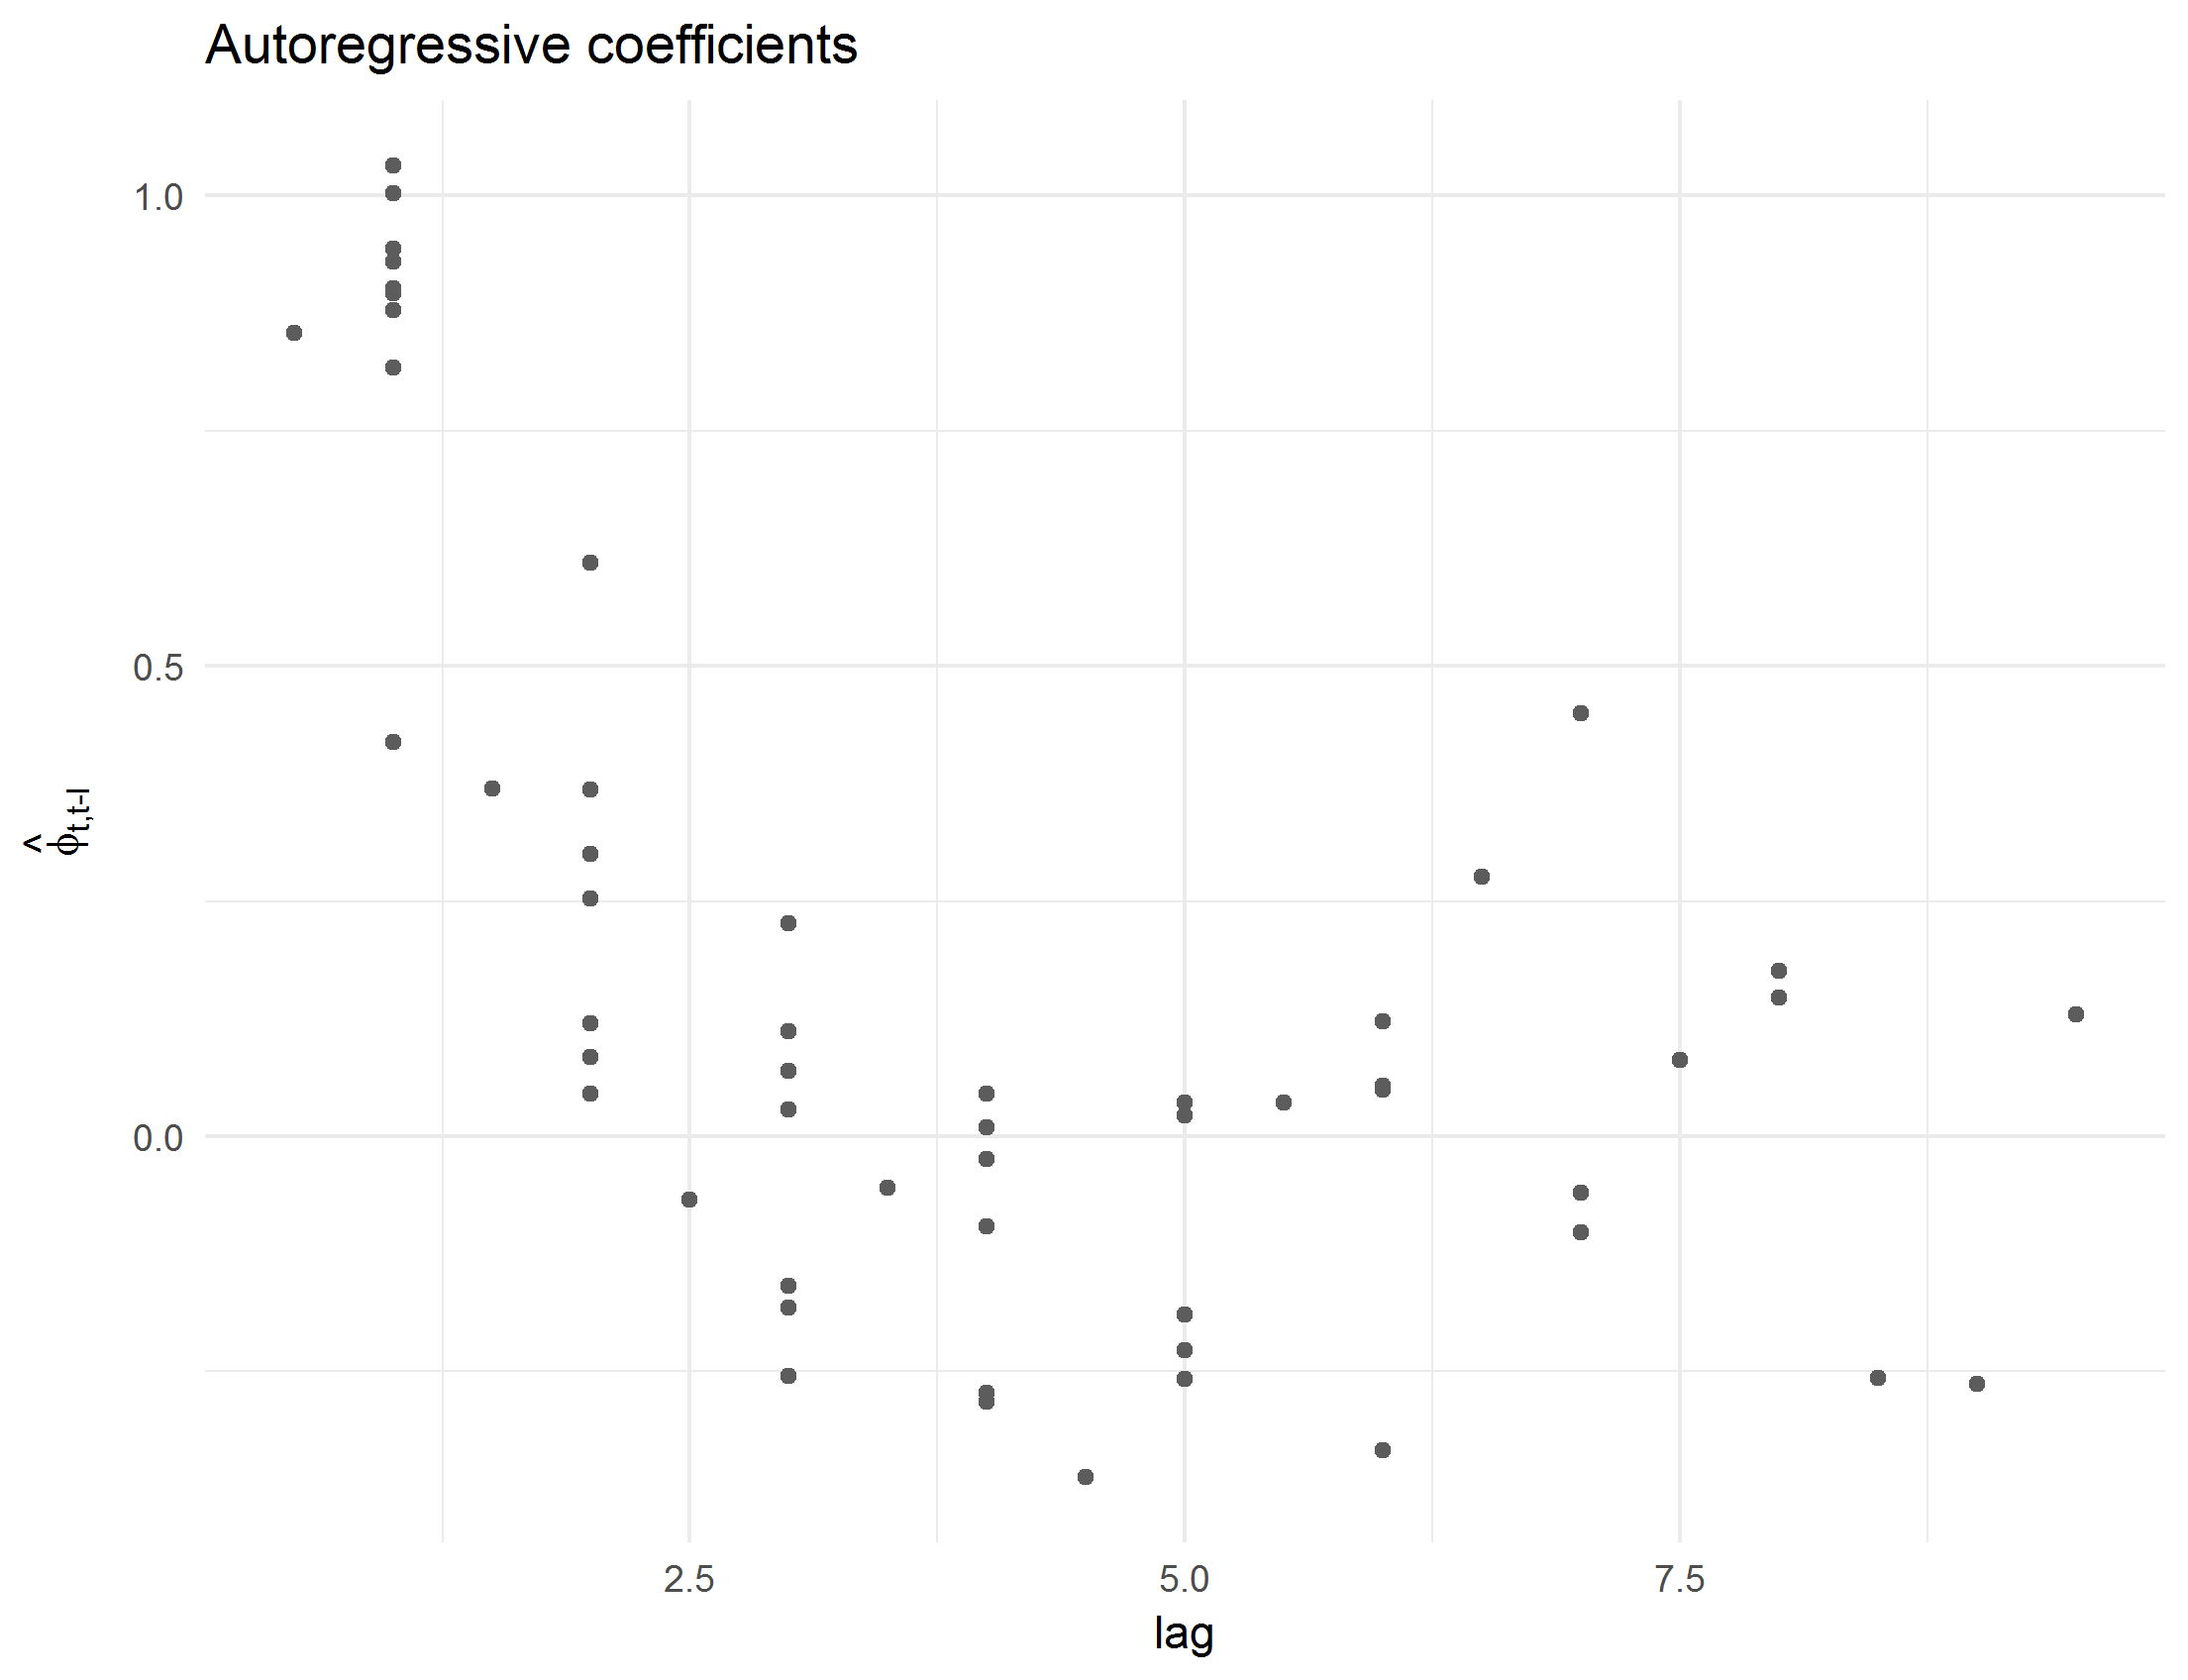
\includegraphics[width = \textwidth]{img/cattle/cattleA-regressogram}
%\end{center}
% \caption{Sample estimates of the generalized autoregressive parameters $\phi_{ij}$ obtained by applying the modified Cholesky decomposition to the sample covariance matrix.}
%\end{figure} 


The analysis of \cite{pourahmadi1999joint} concluded that the regressogram (Figure~\ref{fig:cattleA-regressogram}) and variogram (Figure~\ref{cattleA-innovation-variogram}) suggest that both sample generalised autoregressive parameters and the logarithms of the innovation variances can be characterized in terms of cubic functions of the lag only. They model 

\begin{align}
\begin{split} \label{eq:pourahmadi-cubic-model}
\phi_{ts} = x'_{ts}\gamma, \\
\log\left(\sigma_t^2\right) = z'_{t}\xi, 
\end{split}
\end{align}
\noindent
for $t = 2,\dots, 11$ where 

\begin{align*}
x'_{ts} = \begin{bmatrix} 1 & t - s& \left(t - s\right)^2 & \left(t - s\right)^3 \end{bmatrix},\; \mbox{and } z'_{t} = \begin{bmatrix} 1 & t& t^2& t^3 \end{bmatrix}.
\end{align*}
\noindent
They estimate of $\gamma$ and $\xi$ via maximum likelihood.  Figure~\ref{fig:cattleA-smoothed-regressogram-smoothed-by-t} shows the estimated cubic polynomials corresponding to Model~\ref{eq:pourahmadi-cubic-model}. 


%\begin{figure}[H]
%\centering
%\subfloat[The sample regressogram for the cattle data from treatment group A, overlaid with a cubic polynomial smooth.]{
%  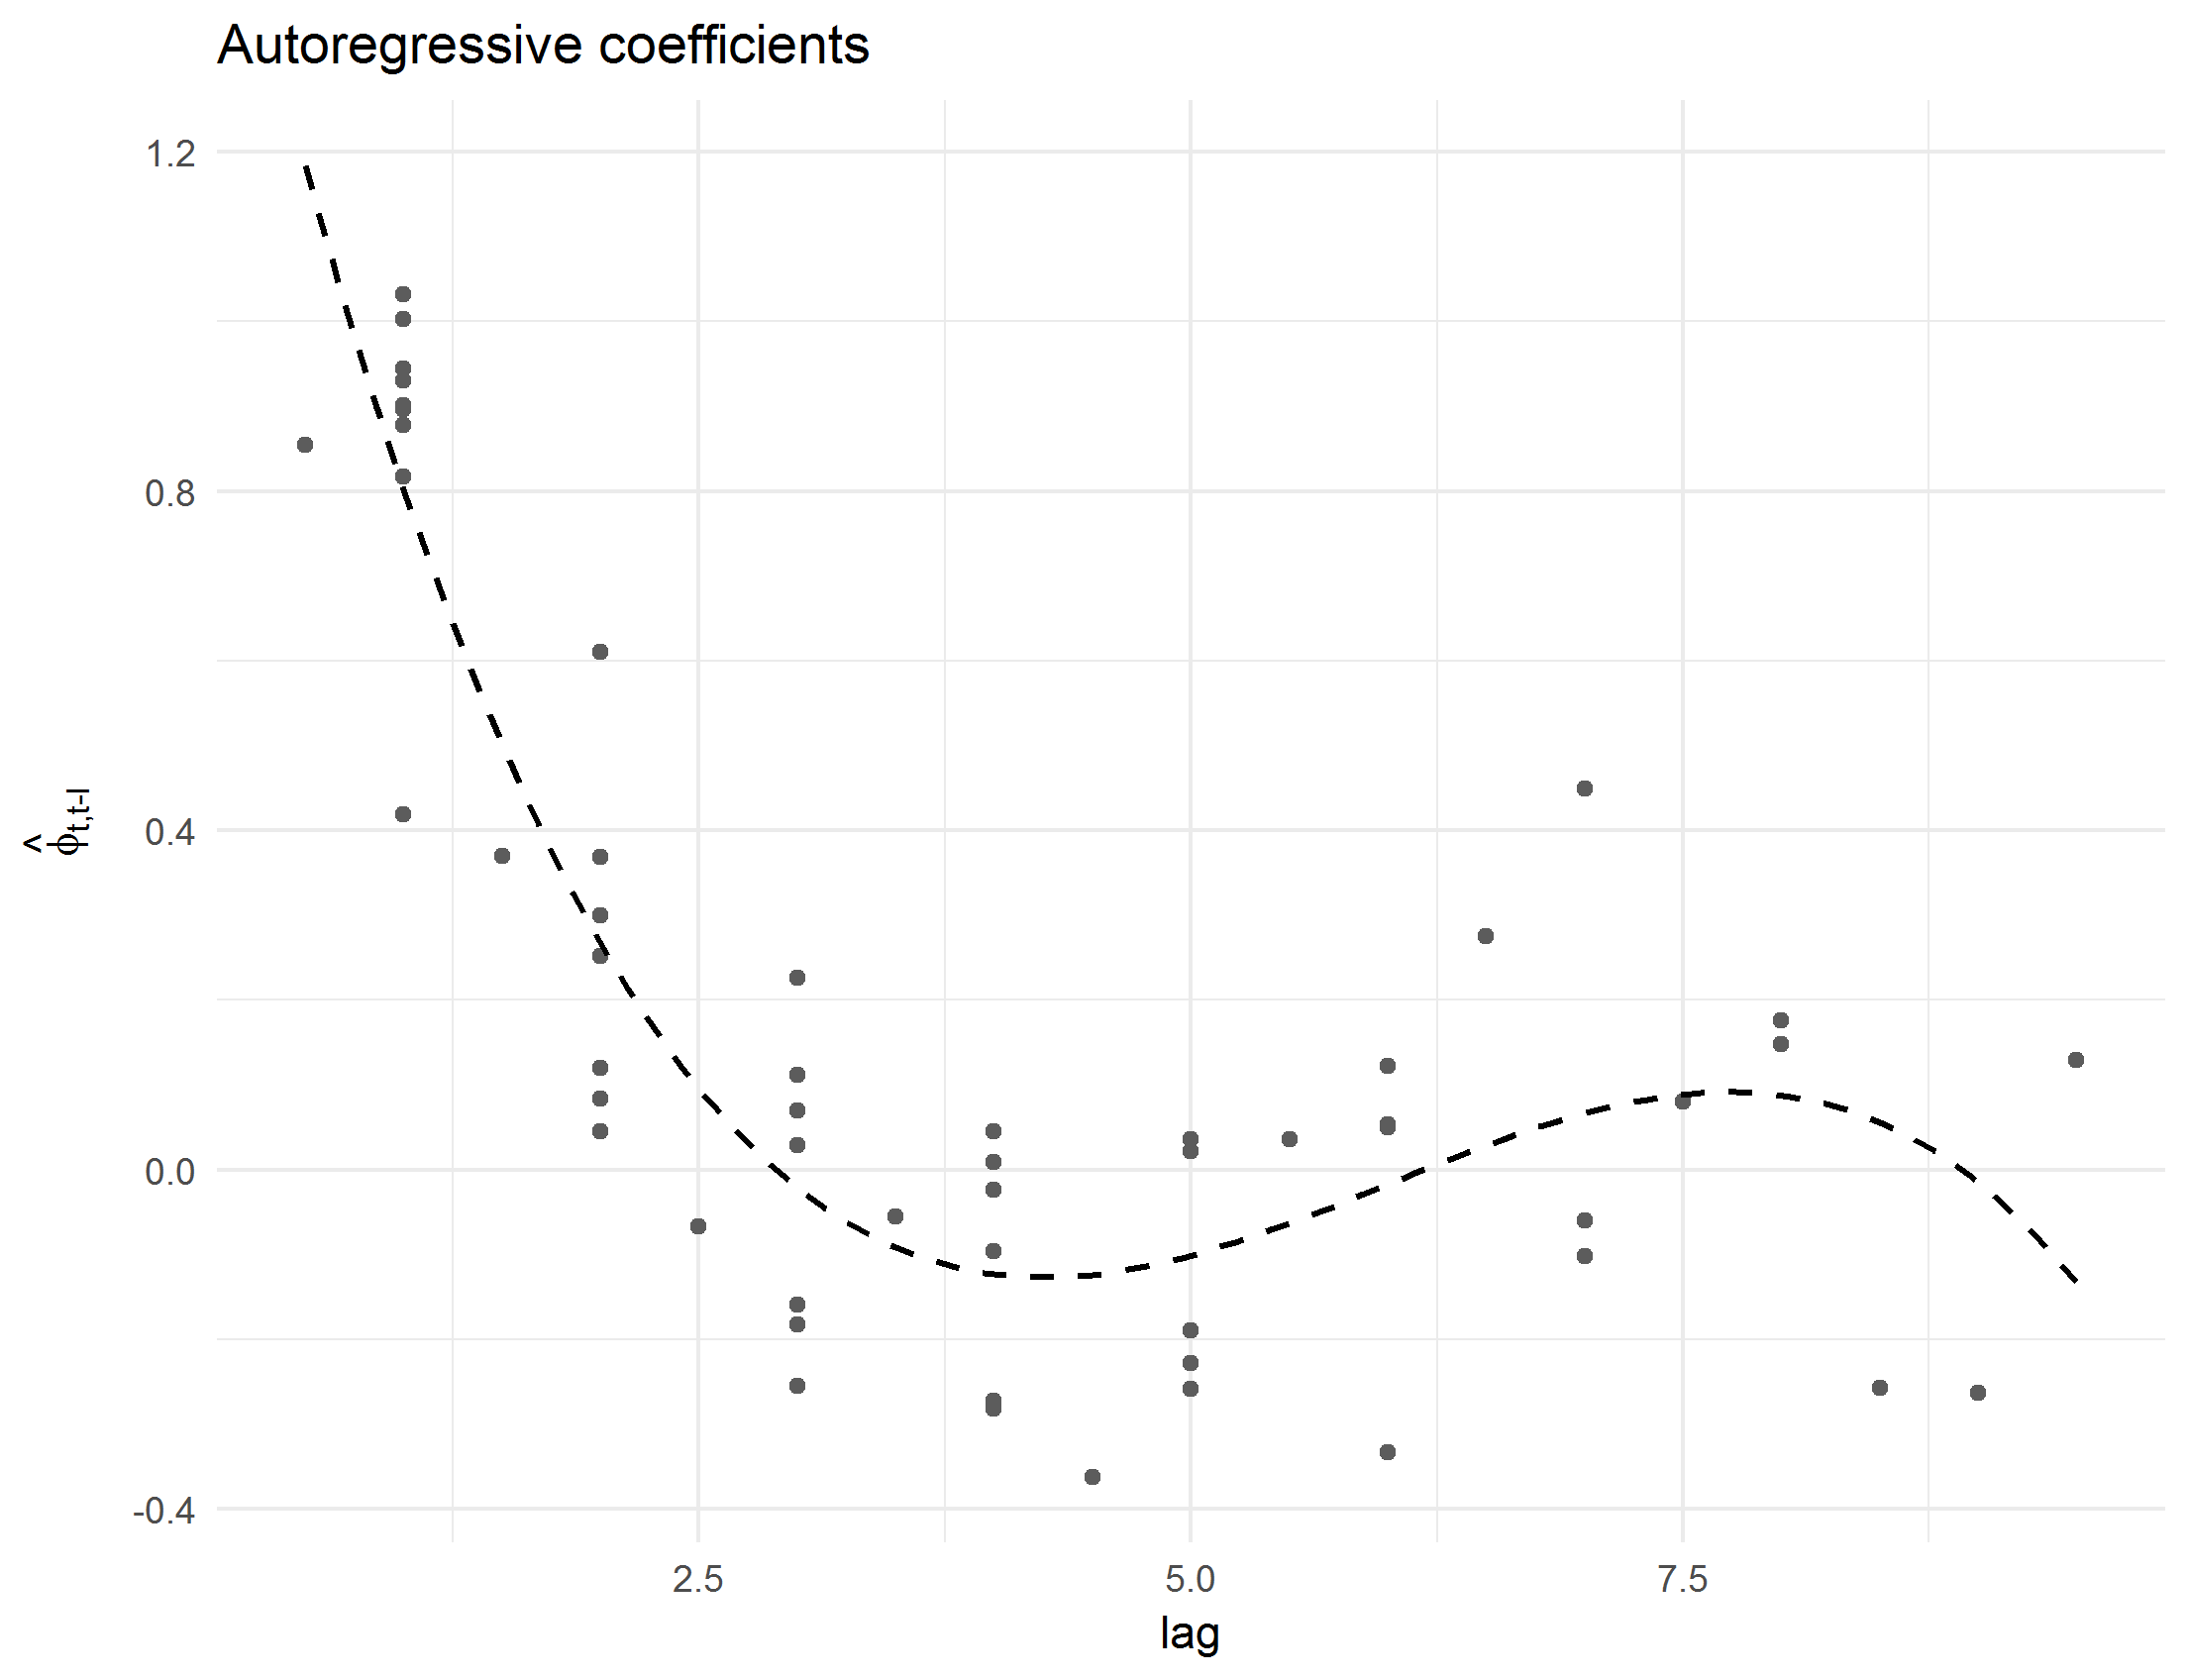
\includegraphics[width = .45\textwidth]{img/cattle/cattleA-regressogram-with-cubic-smooth}\label{fig:cattleA-regressogram-cubic-smooth}
%} 
%\hfill
%\subfloat[The sample variogram for the cattle data from treatment group A, overlaid with a cubic polynomial smooth.]{
%  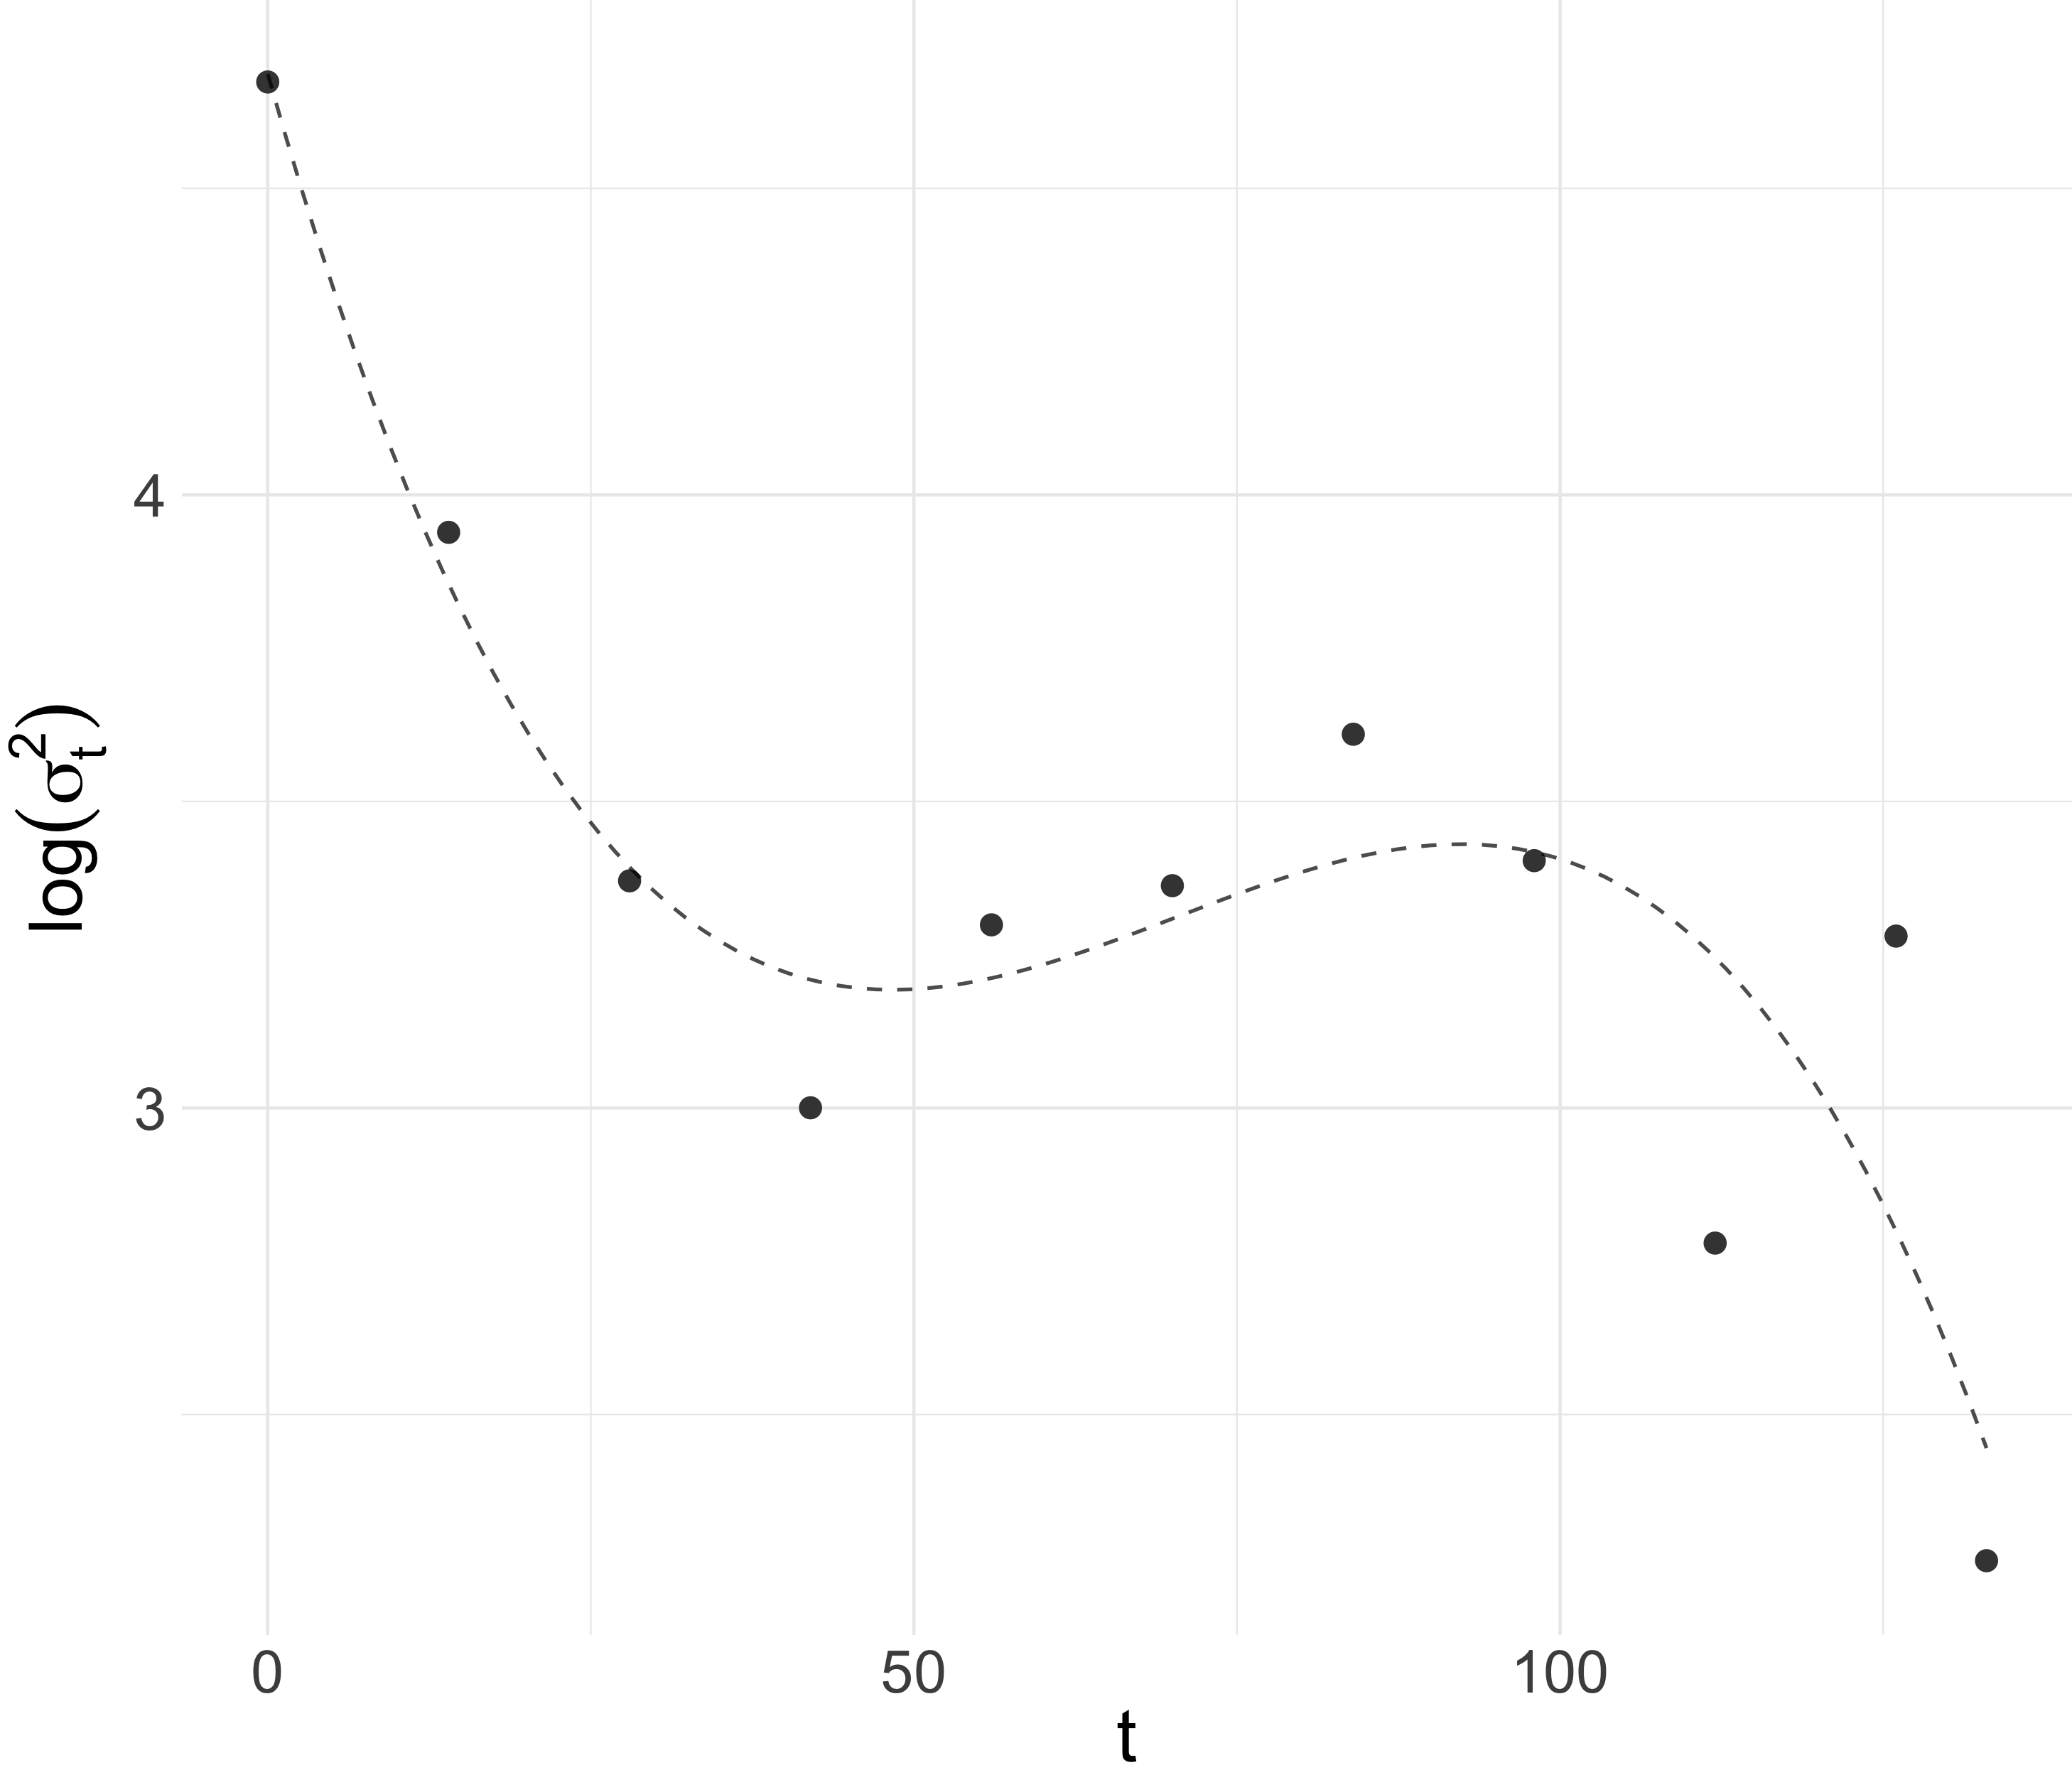
\includegraphics[width = .45\textwidth]{img/cattle/cattleA-innovariogram-with-cubic-smooth}\label{fig:cattleA-innovariogram-cubic-smooth}
%} 
%\end{figure}


\begin{figure}[H]
 \begin{subfigure}{.48\textwidth}
  \centering
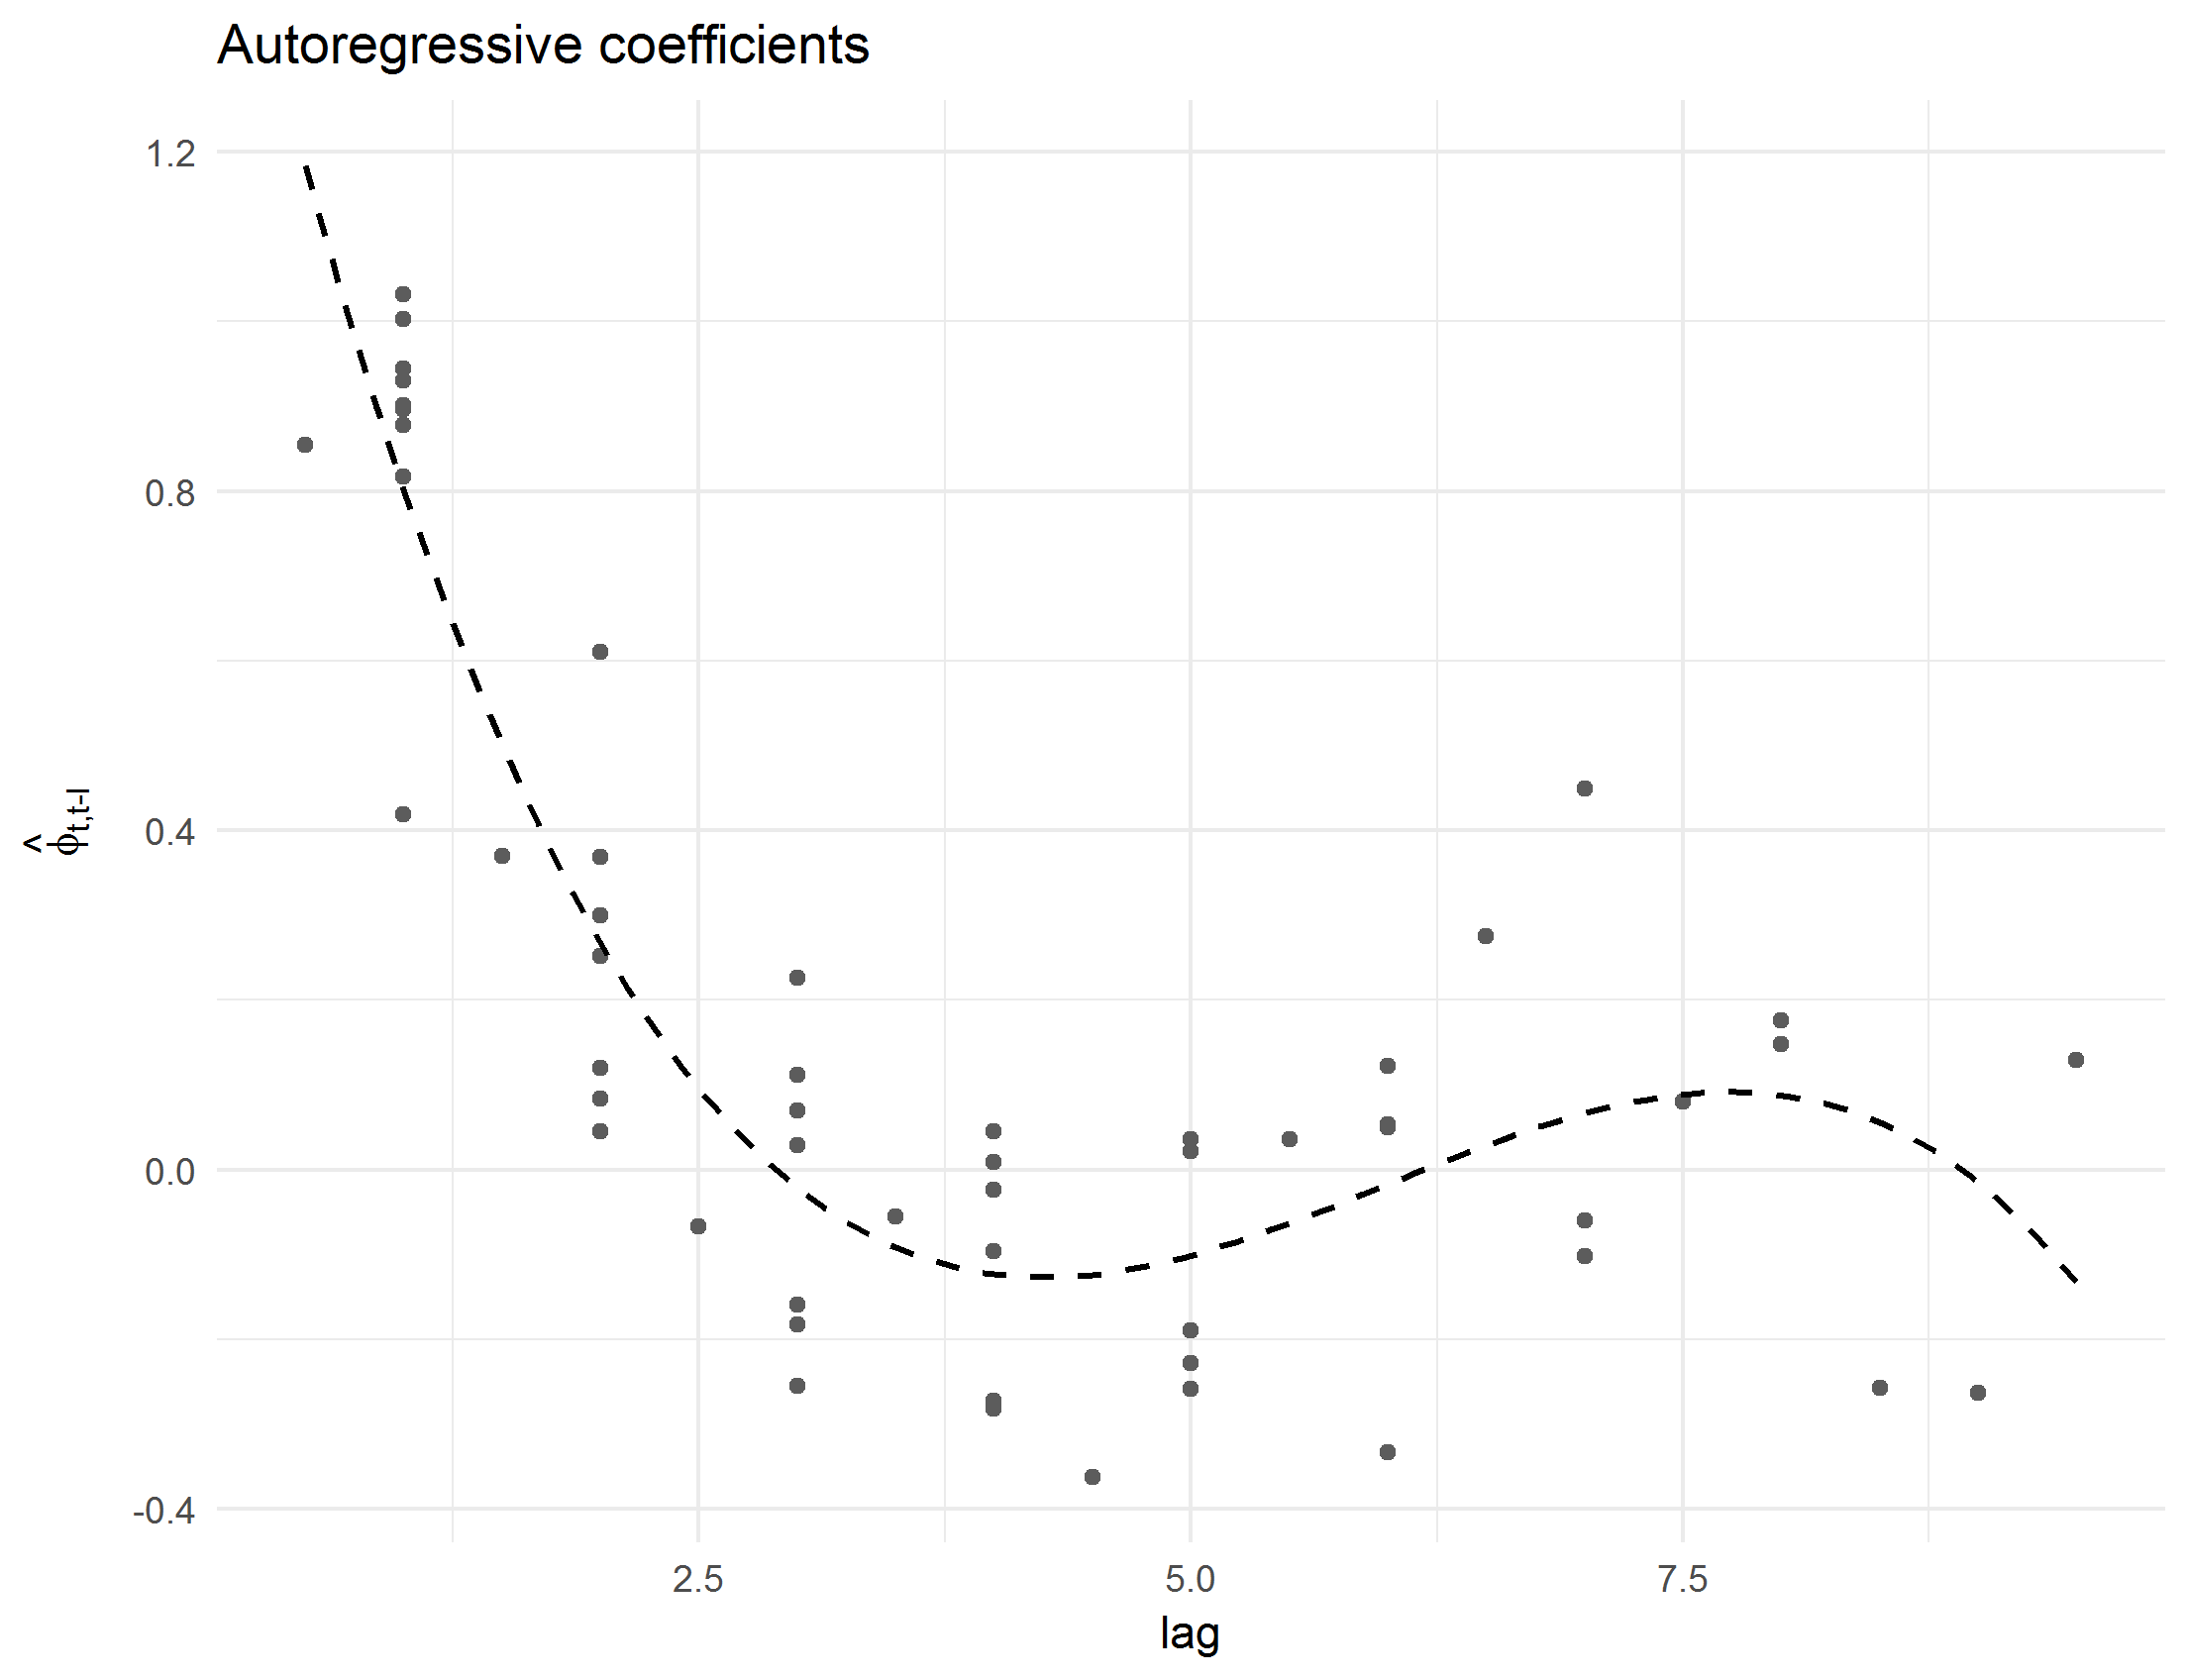
\includegraphics[width = \textwidth]{img/cattle/cattleA-regressogram-with-cubic-smooth}
 \caption{Cubic polynomial fitted to the sample regressogram for the cattle data from treatment group A.} 
 \label{fig:cattleA-innovariogram-cubic-smooth}
 \end{subfigure}
 \begin{subfigure}{.48\textwidth}
  \centering
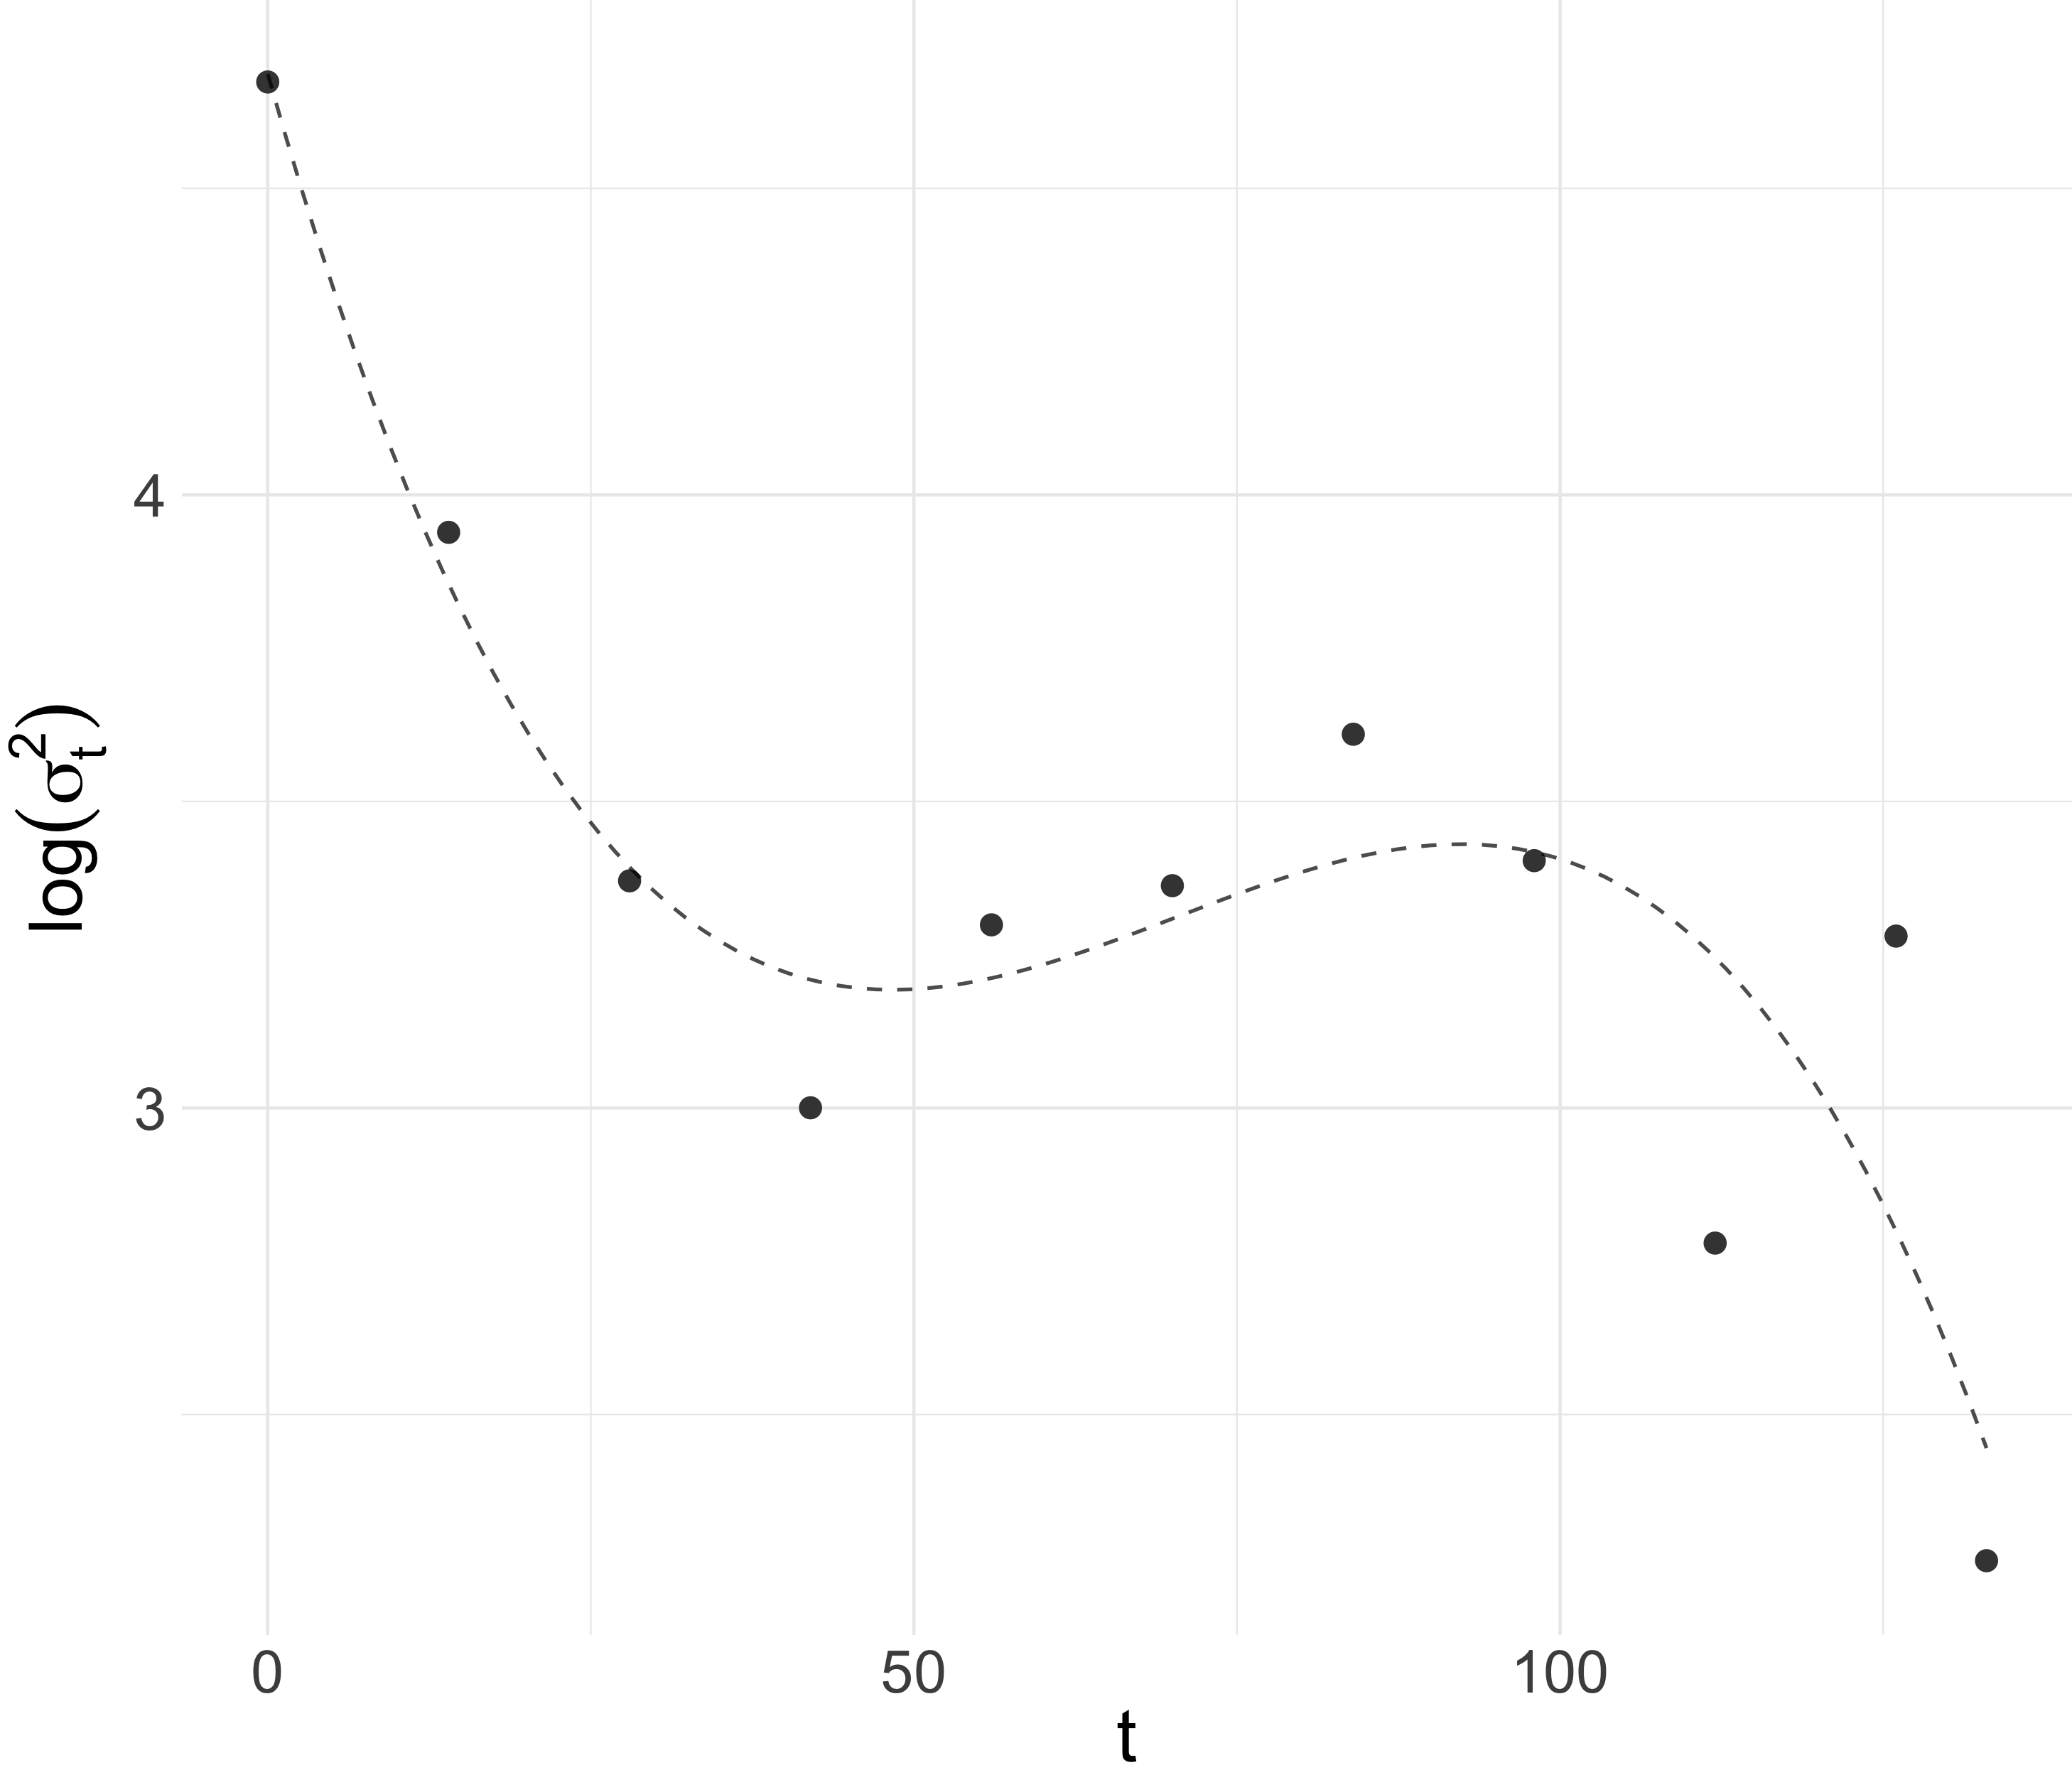
\includegraphics[width = \textwidth]{img/cattle/cattleA-innovariogram-with-cubic-smooth}
 \caption{Cubic polynomial fitted to the sample variogram for the cattle data from treatment group A.} 
\label{fig:cattleA-innovariogram-cubic-smooth}
 \end{subfigure}
% \caption{\textit{Estimated coefficient function} $\hat{\beta}\left(t\right)$ \textit{and mean curve} $\hat{\mu}\left(t\right) = t \sin(2 \pi t)$ \textit{using a 80 B-splines basis functions of order 5 and a difference penalty of order} $k=3$.}
\end{figure}

Choice of penalty is critical for convergence of the iterative estimation of $\phi$ and $\log\left(\sigma_2 \right)$. \cite{pan2017jmcm} concluded that the regressogram of empirical estimates of $\phi_{t,t-l}$ show consistent behaviour over $l$ for each value of $t$, indicating a lack of a strong functional component of $m$. To facilitate a making this modeling decision in an entirely data-driven manner, we let $\phi \in \hilbert = \hilbert_{\left[1\right]} \otimes \hilbert_{\left[2\right]}$, where 

\begin{align*} 
\hilbert_{\left[1\right]} &= \bigg\{ \phi: \ddot{\phi} = 0 \bigg\} \oplus \left\{\phi: \phi\left(0\right) = \dot{\phi}\left(0\right) = 0; \;\; \int\limits_0^1 \ddot{\phi}^2 \;dx < \infty \right\} \\
\hilbert_{\left[2\right]} &= \bigg\{ \phi: \phi \propto 1 \bigg\} \oplus \left\{ \phi: \int\limits_0^1 \phi \;dx = 0, \;\; \dot{f} \in \mathcal{L}_2\left[0,1\right]  \right\} 
\end{align*} 
\noindent
This decomposition leads to a null space comprised of functions of $l$ only, which is attractive because it coincides with the modeling assumptions made by $\phi$ \cite{pan2017jmcm}, \cite{huang2006covariance}, and \cite{wu2003nonparametric} for the same data set.  Figure~\ref{fig:cattle-fitted-cholesky-decomposition} and Figure~\ref{fig:cattle-fitted-cholesky-ssanova} show the estimated Cholesky surface $\phi\left( t,s\right)$ and innovation variance function $\sigma^2\left(t\right)$ evaluated at $t = 1, 2, \dots, 10, 10.5$ and the corresponding pairs of observation times $\left(t,s\right)$, $1 \le s < t \le 10.5$.



\begin{figure}[H]
 \begin{subfigure}{.48\textwidth}
  \centering
  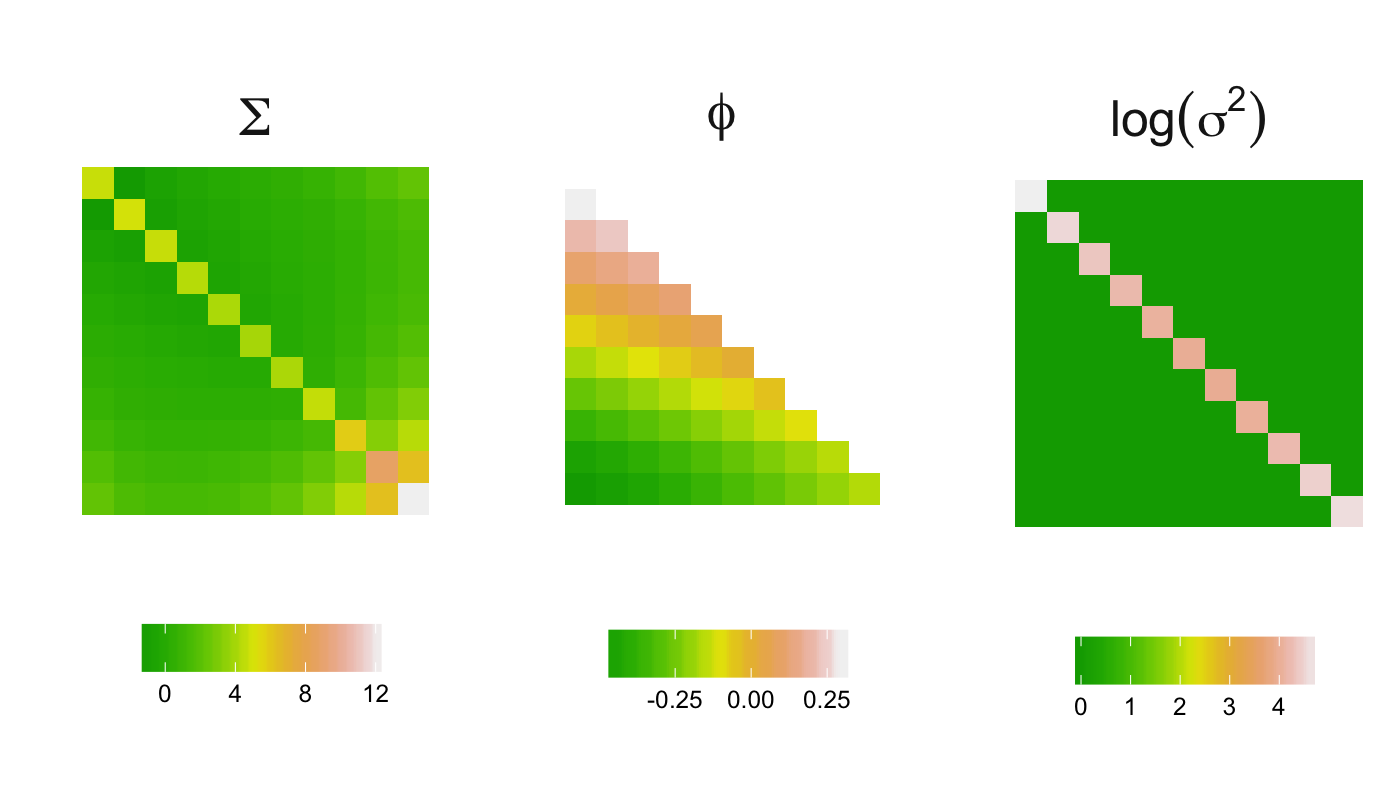
\includegraphics[width = .4\textwidth]{img/chapter-5/cattle-cholesky-estimate-ggplot}
 \caption{Estimated Cholesky factor $\hat{T}$}
 \end{subfigure}
 \begin{subfigure}{.48\textwidth}
  \centering
  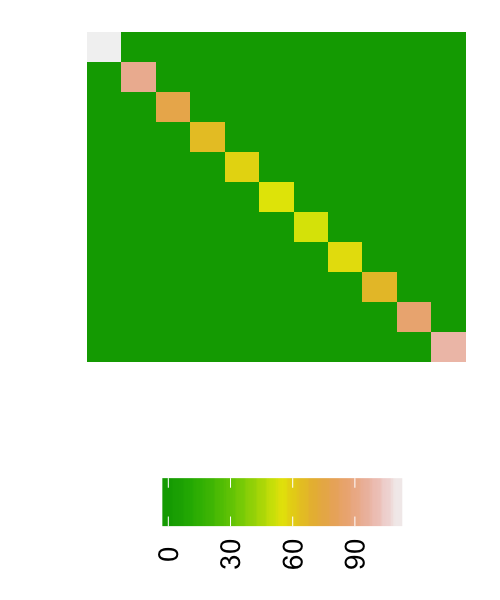
\includegraphics[width = .4\textwidth]{img/chapter-5/cattle-D-estimate-ggplot}
 \caption{Estimated innovation variances \newline $\hat{D} = diag\left( \sigma^2\left(t_1\right),\dots, \sigma^2\left(t_{11}\right) \right)$}
 \end{subfigure}
 \begin{subfigure}{.48\textwidth}
  \centering
  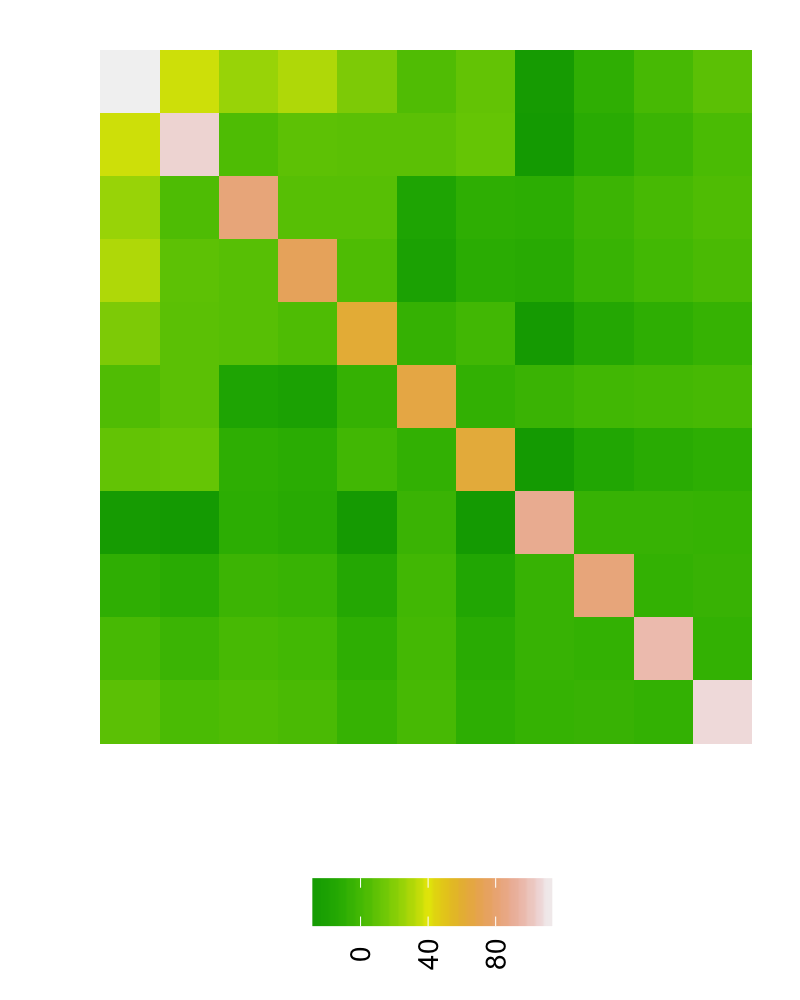
\includegraphics[width = .6\textwidth]{img/chapter-5/cattle-cov-estimate-ggplot}
 \caption{Estimated covariance matrix $\hat{\Sigma} = \hat{T}^{-1} \hat{D} {\hat{T}'}^{-1}$}
 \end{subfigure}
\caption{Components of the fitted modified Cholesky decomposition for the cattle weight data.}
\end{figure}

%%\subfile{chapter-5-subfiles/cattle-cholesky-cov-ggplot}
%\captionsetup[subfigure]{labelformat=empty}
%\begin{figure}[H] 
%\centering
%\caption{Components of the fitted modified Cholesky decomposition for the cattle weight data.}
%\subfloat[Estimated Cholesky factor $\hat{T}$]{
%  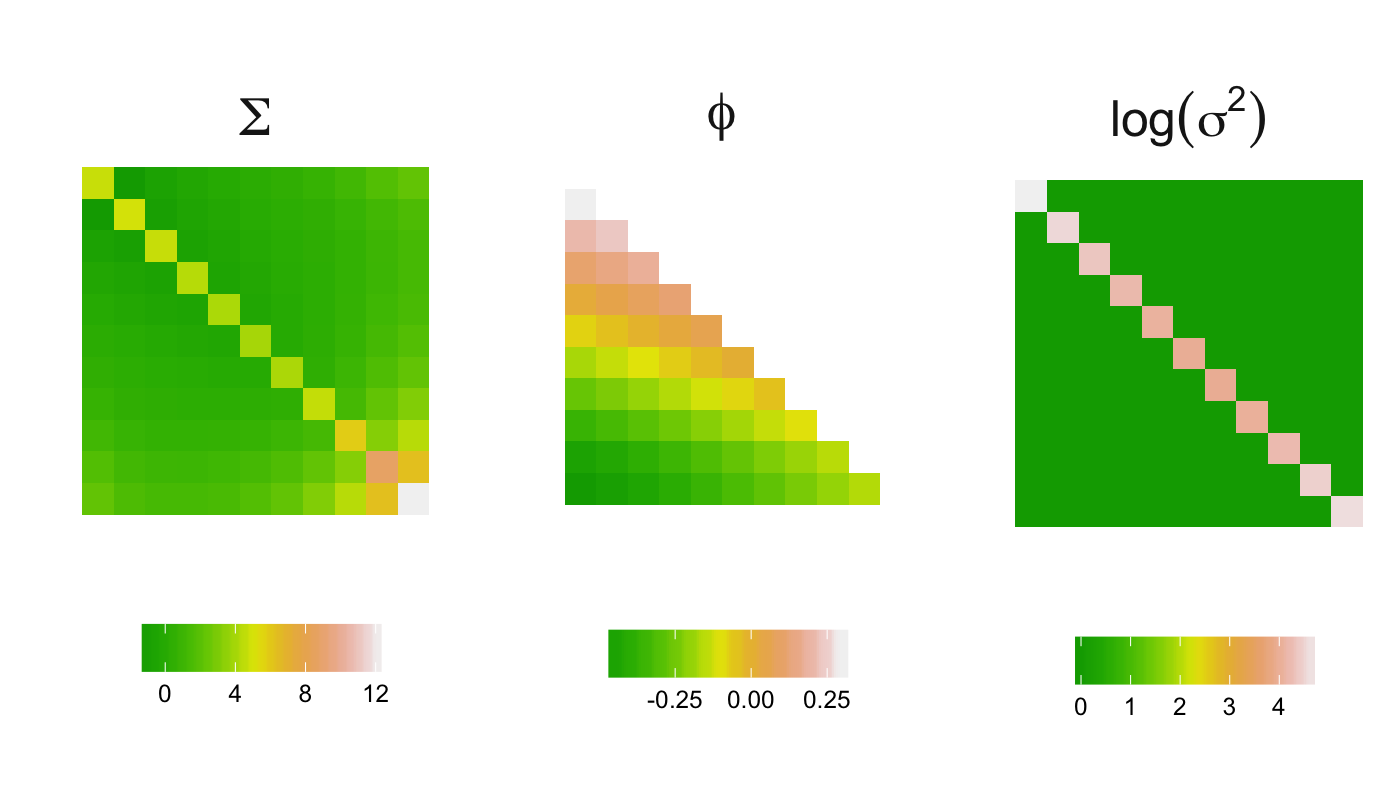
\includegraphics[width = .4\textwidth]{img/chapter-5/cattle-cholesky-estimate-ggplot}
%} \hfill
%\subfloat[Estimated innovation variances \newline $\hat{D} = diag\left( \sigma^2\left(t_1\right),\dots, \sigma^2\left(t_{11}\right) \right)$]{
%  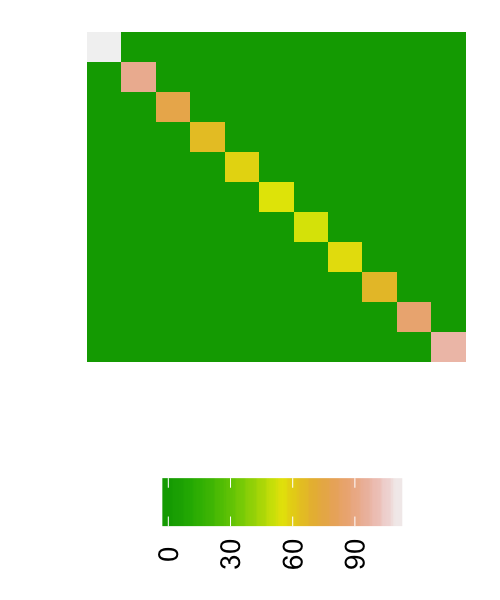
\includegraphics[width = .4\textwidth]{img/chapter-5/cattle-D-estimate-ggplot}
%} 
%\hfill
%\subfloat[Estimated covariance matrix $\hat{\Sigma} = \hat{T}^{-1} \hat{D} {\hat{T}'}^{-1}$]{
%  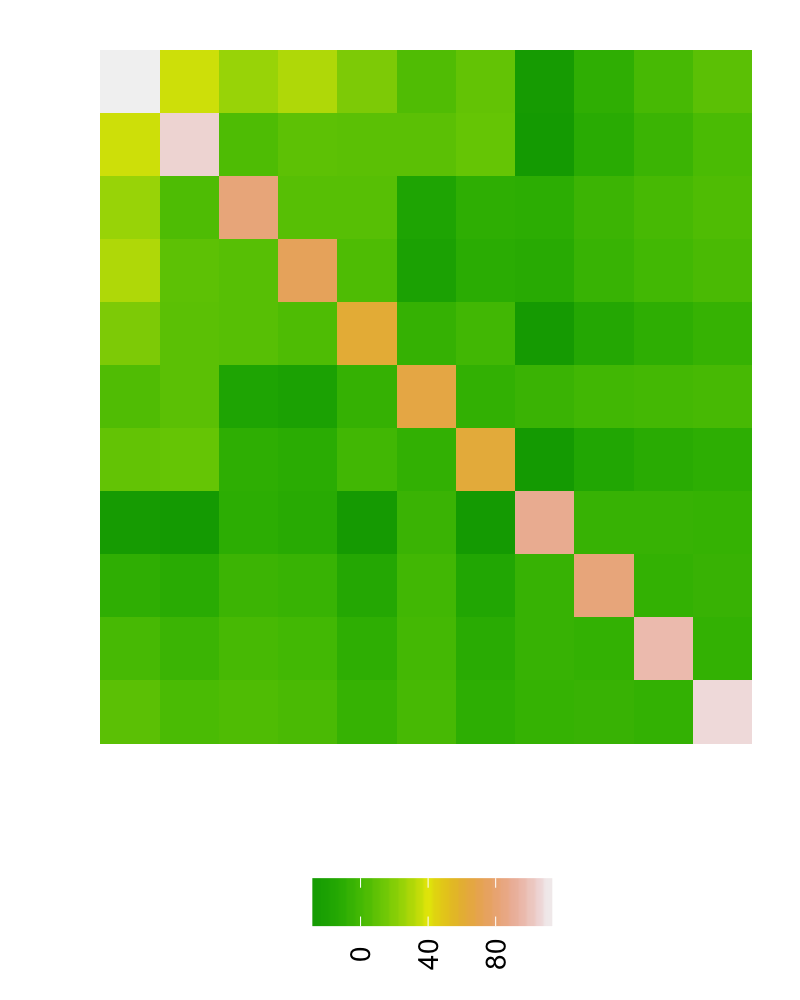
\includegraphics[width = .4\textwidth]{img/chapter-5/cattle-cov-estimate-ggplot}
%} 
%\label{fig:cattle-fitted-cholesky-decomposition}
%\end{figure}

%\subfile{chapter-5-subfiles/cattle-cholesky-ssanova-ggplot}
\begin{figure}[H] 
\centering
\caption{Components of the SSANOVA decomposition of the estimated generalized autoregressive coefficient function $\phi$ evaluated on the grid defined by the observed time points.}
  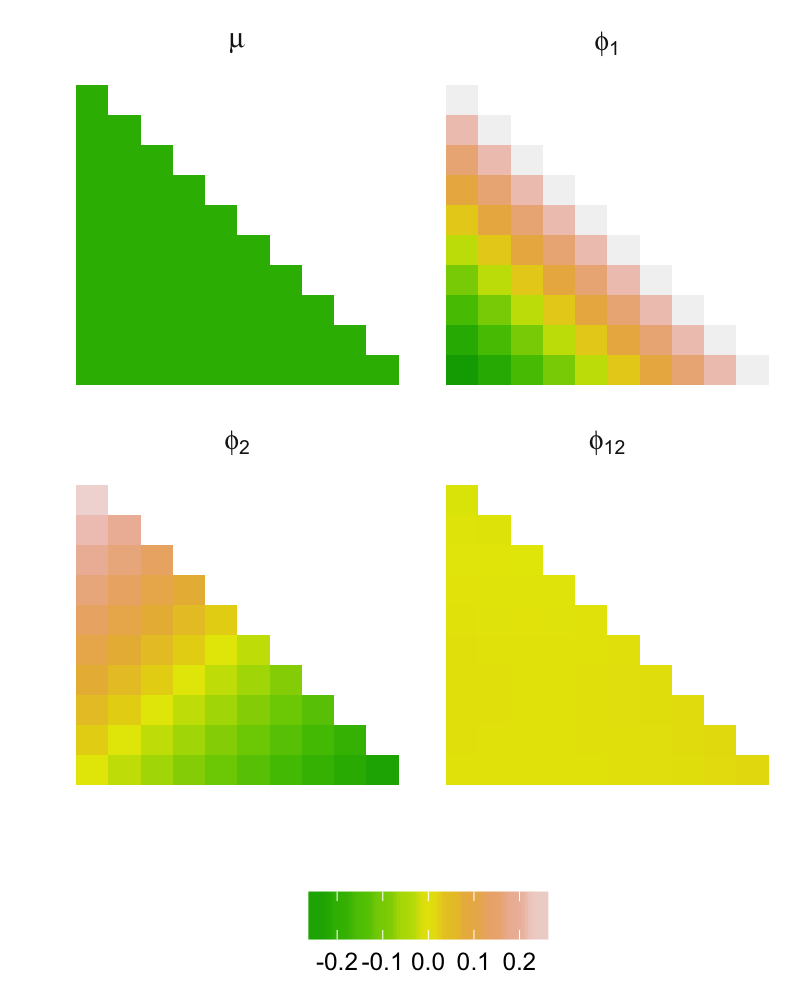
\includegraphics[width = 0.6\textwidth]{img/chapter-5/cattle-ssanova-estimate-lattice} \label{fig:cattle-fitted-cholesky-ssanova}
\end{figure}

Evaluating the normal likelihood at the fitted model gives $\hat{\ell} = -818.5323$.


%\bibliography{../Master}
%
%\end{document}
